\documentclass[preprint,11pt,authoryear]{elsarticle}

%─── Packages ────────────────────────────────────────────────────────────────
\usepackage[T1]{fontenc}
\usepackage[utf8]{inputenc}
\usepackage{lmodern}
\usepackage{amsmath,amssymb,amsthm,bm,bbm}
\usepackage[dvipsnames]{xcolor}
\usepackage{booktabs,colortbl,array,multirow,threeparttable}
\DeclareMathOperator*{\argmin}{arg\,min}
\usepackage{graphicx,float,caption,subcaption}
\graphicspath{{figures/}}
\usepackage{algorithm,algpseudocode}
\usepackage{natbib}
\usepackage{hyperref}
\usepackage{setspace,microtype,enumitem}
\onehalfspacing

%─── Colours ─────────────────────────────────────────────────────────────────
\definecolor{pastelgreen}{rgb}{0.0,0.6,0.0}

%─── Theorem environments ────────────────────────────────────────────────────
\newtheorem{theorem}{Theorem}[section]
\newtheorem{corollary}[theorem]{Corollary}
\newtheorem{definition}[theorem]{Definition}
\newtheorem{remark}[theorem]{Remark}
\newtheorem{assumption}[theorem]{Assumption}
\newtheorem{proposition}[theorem]{Proposition}
\newtheorem{lemma}[theorem]{Lemma}

%─── Notation ────────────────────────────────────────────────────────────────
\newcommand{\VaR}{\mathrm{VaR}}
\newcommand{\ES}{\mathrm{ES}}
\newcommand{\E}{\mathsf{E}}
\renewcommand{\P}{\mathsf{P}}
\newcommand{\1}{\boldsymbol{1}}
\newcommand{\qV}{\hat{q}_{\scriptscriptstyle\mathrm{V}}}
\newcommand{\qE}{\hat{q}_{\scriptscriptstyle\mathrm{E}}}
\newcommand{\EScqr}{\widehat{\ES}^{\,\mathrm{cqr}}}
\newcommand{\CI}{\hat{C}}
\newcommand{\Fhat}{\hat{\mathcal{F}}}
\newcommand{\quantlet}[1]{\href{#1}{\raisebox{-0.15em}{\includegraphics[height=0.9em]{ql_logo.png}}}}
\newcommand{\quantinar}[1]{\href{#1}{\raisebox{-0.15em}{\includegraphics[height=0.9em]{qr_logo.png}}}}

%══════════════════════════════════════════════════════════════════════════════
\begin{document}
	
	\begin{frontmatter}
		
		%─── PART 1: Title and Metadata ──────────────────────────────────────────────
		\title{Distribution-Free Recalibration of Tail Quantile Forecasts\\
			under Temporal Dependence}
		
		% Author details removed for blind review                                         
		
		%─── PART 2: Abstract ───────────────────────────────────────────────────────
		\begin{abstract}
			Tail risk forecasts from heterogeneous models---classical and foundation-model-based---exhibit systematic miscalibration that a single scalar functional can diagnose and correct. This paper proposes a distribution-free recalibration method that adjusts Value-at-Risk forecasts using one-sided conformal prediction, requiring no distributional assumptions or model retraining. An approximate coverage guarantee is established under $\beta$-mixing dependence for the static split-conformal construction. The scalar conformal threshold $\hat{q}_V$ serves both as the corrective shift restoring coverage and as a continuous, signed diagnostic of tail miscalibration severity.

			The method is evaluated on five time series foundation models and four classical benchmarks across 24 financial assets over 2000--2026. Conformal recalibration empirically restores nominal coverage across a wide range of model--asset combinations, achieving broad Basel Green Zone compliance with the static split---stronger among model--asset pairs where the base forecast retains predictive content---and near-full compliance with the rolling variant, revealing a calibration--efficiency trade-off. The results establish that forecast validity can be separated from forecast generation: a one-parameter, distribution-free post-processing layer empirically restores tail coverage without modifying the underlying predictive model.

			\bigskip\noindent
			\textbf{Keywords:} Conformal prediction; probabilistic forecast calibration; Value at Risk; time series foundation models; distribution-free recalibration; temporal dependence; quantile score

			\bigskip\noindent
			\textbf{JEL:} C14\,|\,C53\,|\,C58\,|\,G17\,|\,G32
		\end{abstract}
		
	\end{frontmatter}
	
	%══════════════════════════════════════════════════════════════════════════════
	%─── PART 4: Introduction ───────────────────────────────────────────────────
	%══════════════════════════════════════════════════════════════════════════════
	\section{Introduction}
	\label{sec:intro}

	Accurate calibration of tail risk forecasts remains a central challenge in forecasting under temporal dependence. Empirical evidence across financial markets shows that even state-of-the-art models---ranging from parametric volatility specifications to modern time series foundation models---systematically misestimate extreme quantiles, leading to violations of nominal coverage and unreliable risk assessment \citep{christoffersen1998, nolde2017elicitability, goel2024tsfmvar, pele2025llmvar}. The problem is particularly acute in the lower tail, where the effective sample size is intrinsically limited and where Value-at-Risk (VaR) forecasts are subject to formal regulatory backtesting \citep{basel1996} whose failures translate directly into capital penalties.

	This paper starts from a simple but underexplored observation: at tail probability level $\alpha$ with $T$ test observations, the number of informative tail events is of order $O(\alpha T)$. For typical applications ($\alpha = 0.01$, $T \approx 1{,}500$), only a handful of observations effectively determine tail calibration. In such regimes, high-dimensional recalibration procedures are statistically unstable, as variance inflation dominates any potential bias reduction. The appropriate complexity class for tail recalibration under dependence is therefore inherently low-dimensional; this principle, formalized in Proposition~\ref{prop:tail_sparsity}, is the backbone of the paper.

	We study a one-parameter, model-agnostic recalibration rule based on one-sided conformal prediction: a scalar shift applied to predicted lower quantiles, estimated from past forecast errors. Although minimal in form, this correction is shown to be statistically well-suited to the tail sparsity constraint across a wide range of forecasting models and asset classes. Crucially, the correction term itself---the conformal threshold $\qV$ (Definition~\ref{def:var_correction})---admits a natural interpretation as a continuous, signed measure of tail misspecification. It explains a substantial fraction of the cross-sectional variation in forecast performance (partial $R^2 = 54.6\%$; Section~\ref{sec:results_raw}) and anticipates backtesting failures, thereby extending the role of recalibration from a corrective device to a tool for model assessment.

	On the theoretical side, we establish an asymptotic coverage result for the static split-conformal procedure under $\beta$-mixing dependence (Theorem~\ref{thm:dependent_conformal_var}). This result provides formal support for the direction of the correction but does not extend to the rolling implementation used in practice; empirical validity of the rolling variant is demonstrated separately. The empirical evaluation covers five time series foundation models (TSFMs), four parametric benchmarks, and 24 financial assets over 2000--2026. This constitutes a systematic calibration audit of time series foundation models for financial tail risk---the broadest to date in terms of model diversity (five architectures), asset coverage (24 series across five classes), and sample length---using Kupiec, Christoffersen, and Basel traffic-light tests. Conformal extensions to Expected Shortfall, which lacks the elicitability structure of VaR \citep{gneiting2011making}, are discussed in Section~\ref{sec:discuss} and Appendix~\ref{app:es}.

	The contribution of the paper is therefore not the introduction of a new conformal algorithm, but the identification of the appropriate statistical complexity class for tail recalibration under dependence. A one-parameter adjustment achieves a favourable bias--variance trade-off in sparse tail regimes, while more flexible alternatives---isotonic regression, multi-parameter recalibration, adaptive conformal inference---either overfit or trade sharpness for coverage on a calibration--efficiency frontier (Table~\ref{tab:baselines}). The work belongs to the forecast post-processing tradition of \citet{gneiting2013combining}, \citet{brehmer2021properification}, and \citet{taillardat2016calibrated}, focusing specifically on tail risk measures under dependence.

	% Data and code availability: removed for blind review
	
	%══════════════════════════════════════════════════════════════════════════════
	%─── PART 5: Literature Review ──────────────────────────────────────────────
	%══════════════════════════════════════════════════════════════════════════════
	\section{Related Literature}
	\label{sec:lit}
	
	This paper connects three strands of the forecasting literature:
	foundation models for financial time series, regulatory
	evaluation of tail risk forecasts, and distribution-free
	calibration via conformal prediction.
	
	Recent TSFMs---including Chronos
	\citep{ansari2024chronos,ansari2025chronos2}, TimesFM
	\citep{das2024timesfm}, Moirai
	\citep{woo2024moirai,liu2024moirai2}, and Lag-Llama
	\citep{rasul2024lagllama}---achieve competitive zero-shot
	accuracy but produce miscalibrated tail forecasts.
	\citet{goel2024tsfmvar} show that pre-trained quantiles
	require fine-tuning for acceptable VaR coverage,
	\citet{rahimikia2025revisiting} document systematic
	miscalibration across financial datasets, and
	\citet{pele2025llmvar} highlight tail compression in
	instruction-tuned models. These findings motivate post-hoc
	correction approaches. This study provides a systematic
	calibration audit of time series foundation models for financial
	tail risk---the broadest to date in terms of model diversity, covering five architectures across 24 assets over a
	quarter-century sample.

	Established backtesting procedures---unconditional coverage
	\citep{kupiec1995}, conditional coverage
	\citep{christoffersen1998}, the Basel Traffic Light
	\citep{basel1996}, the $Z_2$ test for ES
	\citep{acerbi2014back}, and the joint elicitability framework
	of \citet{fissler2016higher} and
	\citet{nolde2017elicitability}---diagnose miscalibration but
	do not prescribe a correction. Comparative evaluation relies
	on the Diebold--Mariano framework
	\citep{diebold1995comparing,harvey1997testing}. This
	limitation motivates calibration procedures that operate
	directly on forecast outputs.
	
	To address this limitation, the post-processing paradigm adjusts
	the output of a fixed forecaster without retraining
	\citep{gneiting2013combining, brehmer2021properification,
		taillardat2016calibrated}. Model-based
	alternatives such as CAViaR \citep{engle2004caviar} estimate
	conditional quantiles directly but require specification of
	the underlying process.
	
	Conformal prediction \citep{vovk2005algorithmic}, extended to
	quantile regression by \citet{romano2019conformalized},
	provides a distribution-free calibration framework. A central
	challenge for financial applications is temporal dependence:
	exchangeability of the nonconformity scores is violated under volatility clustering.
	Existing approaches address this through weighted conformal
	methods \citep{barber2023conformal}, blocking schemes
	\citep{chernozhukov2018exact}, or sequential procedures
	\citep{gibbs2021adaptive, zaffran2022conformal,
		xu2024conformal}, often at the cost of increased complexity.
	This paper adopts a simple split conformal framework with
	explicit remainder bounds under $\beta$-mixing dependence,
	drawing on empirical process theory
	\citep{rio2017asymptotic, yu1994rates}, and reinterprets the
	conformal correction as a diagnostic object that measures both
	the magnitude and direction of tail miscalibration.
	
	%══════════════════════════════════════════════════════════════════════════════
	%─── PART 6: Framework ──────────────────────────────────────────────────────
	%══════════════════════════════════════════════════════════════════════════════
	\section{Framework}
	\label{sec:framework}
	
	We consider a two-layer forecasting framework. A base model
	produces probabilistic forecasts of returns, while a separate
	calibration layer adjusts these forecasts to ensure correct
	coverage of tail risk measures. The objective is not to modify
	the underlying model, but to restore the reliability of its
	predicted quantiles through a minimal post-processing step.
	
	We use the following notation throughout. Let $r_t$ denote the
	daily log return and $\hat{q}_t^{lo}$ the predicted lower
	$\alpha$-quantile from a base model $M$. The one-sided
	nonconformity score is $s_t^{V} = \hat{q}_t^{lo} - r_t$. The
	conformal threshold is
	$\qV = Q_{1-\alpha}(\{s_t^{V}\})$, the empirical
	$(1-\alpha)$-quantile of the calibration scores. The
	conformally corrected Value-at-Risk is
	$\widehat{\VaR}_t^{\,\mathrm{cp}} = \qV - \hat{q}_t^{lo}$.
	Finally, $\hat{q}_{V,t}^{\mathrm{roll}}$ denotes the
	rolling-window version.
	Throughout the paper, we use $\alpha = 0.01$ interchangeably with a 1\% tail probability (99\% coverage level).
	We use $\VaR_t$ generically when no ambiguity arises, and superscripts (raw, cp, roll) to distinguish variants where necessary. All VaR values are reported as positive loss thresholds; the corresponding quantile is $\hat{q}_t = -\VaR_t$.

	\subsection{TSFM-VaR Setup}
	\label{sec:setup}
	
	A foundation model $M$ generates a probabilistic forecast for
	the next-period return. For sample-based models (Chronos,
	Moirai, Lag-Llama), the forecast consists of $N=1{,}000$ draws
	obtained via ancestral or mixture-distribution sampling,
	forming the empirical predictive CDF
	\[
	\Fhat_t^M(x) = \frac{1}{N}\sum_{i=1}^{N}
	\1(\hat{r}_t^{i;M}\leq x).
	\]
	Value-at-Risk and Expected Shortfall are computed following
	\citet{pele2025llmvar}:
	\begin{align}
		\widehat{\VaR}_t^{\alpha;M}
		&= -(\Fhat_t^M)^{-1}(\alpha), \\
		\widehat{\ES}_t^{\alpha;M}
		&= -\frac{1}{\lfloor N\alpha\rfloor}
		\sum_{k=1}^{\lfloor N\alpha\rfloor}\hat{r}_{t,(k)}^M,
	\end{align}
	where $\hat{r}_{t,(k)}^M$ denotes the $k$-th order statistic.
	This is the empirical analogue of
	$\ES_\alpha = -\frac{1}{\alpha}\int_0^\alpha F^{-1}(u)\,du$;
	the approximation is exact as $N \to \infty$.
	For the baseline configuration ($N = 1{,}000$,
	$\alpha = 0.01$), the sum uses $\lfloor N\alpha \rfloor = 10$
	order statistics, yielding a coefficient of variation of
	approximately $1/\sqrt{10} \approx 0.32$, compared with
	$O(1/\sqrt{N})$ for the median. This motivates our focus on
	VaR for the formal conformal analysis.
	For quantile-based models (e.g., TimesFM), VaR is given
	directly by the predicted $\alpha$-quantile; when required
	levels are not available, a parametric interpolation is applied
	within the base pipeline. For parametric benchmarks
	(GJR-GARCH, GARCH-Normal, Historical Simulation, EWMA), VaR
	and ES are computed from the model's conditional distribution
	with a 250-day rolling estimation window.
	
	\subsection{Diagnosing Miscalibration}
	\label{sec:diag}
	
	We evaluate calibration using standard regulatory backtesting
	procedures. Let $\alpha_{\mathrm{VaR}} = 0.01$ and define the
	violation indicator
	$V_t = \1(r_t < -\widehat{\VaR}_t^{\alpha;M})$. The
	\citet{kupiec1995} likelihood ratio test evaluates
	unconditional coverage:
	\begin{equation}
		\label{eq:kupiec}
		\mathrm{LR}_{\mathrm{POF}} = -2\ln\!\left\{
		\frac{(1-\alpha)^{N-x}\alpha^x}
		{(1-x/N)^{N-x}(x/N)^x}\right\}
		\;\sim\; \chi^2_1,
	\end{equation}
	where $x = \sum_t V_t$. The Basel Traffic Light
	\citep{basel1996} classifies models into Green, Yellow, and
	Red zones based on violation counts. To assess tail severity,
	we use the $Z_2$ statistic of \citet{acerbi2014back}:
	\begin{equation}
		\label{eq:Z2}
		Z_2 = \sum_{t=1}^N
		\frac{I_t\, r_t}{N\alpha\,\widehat{\ES}_t^\alpha} + 1,
	\end{equation}
	where $I_t = \1(r_t \leq -\widehat{\VaR}_t^\beta)$ with $\beta = \alpha$. These
	diagnostics detect miscalibration but do not quantify its
	magnitude or provide a correction mechanism.
	To complement backtesting diagnostics with a joint scoring perspective, we also consider evaluation of Value-at-Risk and Expected Shortfall using the Fissler--Ziegel (FZ) scoring framework \citep{fissler2016higher}, which is strictly consistent for the pair (VaR, ES). Given that the ES component in our framework is obtained via a heuristic correction (Appendix~\ref{app:es}), FZ scores are interpreted as diagnostic rather than as a formal validation criterion; empirical results are reported in Section~\ref{sec:forecast_eval} and Table~\ref{tab:fz_scores}.

	\subsection{One-Sided Conformal VaR Correction}
	\label{sec:cqr_var}
	
	Conformal prediction is a distribution-free calibration
	framework that adjusts forecasts using held-out residuals to
	achieve guaranteed coverage
	\citep{vovk2005algorithmic, romano2019conformalized}. We
	adapt this idea to one-sided tail risk: rather than
	constructing a symmetric prediction interval, we shift the
	predicted VaR by a constant amount such that past forecast
	errors achieve the desired coverage level.
	
	The forecast outputs are split temporally into a calibration
	set and a test set. No forecasts are re-estimated. The
	calibration fraction is fixed at $f_c = 0.70$, with
	robustness examined in Section~\ref{sec:robust}.
	
	\begin{definition}[One-Sided VaR Nonconformity Score]
		\label{def:var_score}
		The nonconformity score measures how far each realised
		loss falls beyond the predicted quantile:
		\begin{equation}
			s_t^{\mathrm{V}} = \hat{q}_t^{lo} - r_t,
		\end{equation}
		where $\hat{q}_t^{lo} = (\Fhat_t^M)^{-1}(\alpha)$. The
		score is positive when the realised loss exceeds the
		predicted quantile, measuring the extent of risk
		underestimation.
	\end{definition}
	
	The conformal correction selects the quantile of these scores
	that restores nominal coverage on the calibration set.
	
	\begin{definition}[Conformal VaR Correction]
		\label{def:var_correction}
		The conformal threshold is the $(1-\alpha)$-quantile of
		the calibration scores, and the corrected VaR is obtained
		by shifting the base quantile:
		\begin{align}
			\qV &= Q_{1-\alpha}(\{s_t^{\mathrm{V}}\}), \\
			\widehat{\VaR}_t^{\,\mathrm{cp}}
			&= \qV - \hat{q}_t^{lo}. \label{eq:var_cp}
		\end{align}
		Since $\hat{q}_t^{lo} < 0$, the corrected quantile level is $\hat{q}_t^{lo} - \qV$ (more negative when $\qV > 0$, i.e., wider coverage), and $\widehat{\VaR}_t^{\,\mathrm{cp}} = -(\hat{q}_t^{lo} - \qV) > 0$ reports the VaR as a positive loss threshold.
		The scalar $\qV$ shifts the predicted quantile to restore
		nominal coverage in the calibration sample; its role is not to introduce new predictive structure, but to correct systematic miscalibration in the existing forecast. Larger values indicate systematic
		underestimation of risk, while negative values reflect
		over-conservative forecasts. Among all constant
		adjustments, $\qV$ minimises the pinball loss on the
		calibration set: $\argmin_c \sum_t
		\rho_{1-\alpha}(s_t^V - c) = Q_{1-\alpha}(\{s_t^V\})$,
		the standard result that the quantile minimises the check
		loss \citep[Theorem~1.1]{koenker2005quantile}.
	\end{definition}

	\paragraph{Notation summary.}
	Throughout, $\widehat{\VaR}^{\,\mathrm{raw}}_t$ denotes the uncorrected base forecast, $\widehat{\VaR}^{\,\mathrm{cp}}_t$ the static conformally corrected forecast (eq.~\ref{eq:var_cp}), $\widehat{\VaR}^{\,\mathrm{roll}}_t$ the rolling corrected forecast (eq.~\ref{eq:var_roll}), and $\widehat{\VaR}^{\,\mathrm{sc}}_t$ the scale-corrected baseline (Table~\ref{tab:baselines}).

	We report $\widehat{\VaR}_t^{\,\mathrm{cp}}$ as the corrected quantile level (expressed in quantile form) induced by the conformal shift, preserving standard VaR interpretation.
	The correction restores violation frequency but does not
	modify the shape of the predictive distribution. This design
	prioritises robustness over flexibility: a one-parameter
	correction avoids overfitting in the sparse tail region. A
	heuristic ES correction is provided in
	Appendix~\ref{app:es}.
	
	\begin{remark}[Relation to properification]
		The conformal correction is a special case of the
		\citet{brehmer2021properification} properification framework:
		it is the identity properification map restricted to location
		shifts, $T(q) = q + c$ with $c = \qV$. This additive
		adjustment maps a potentially improper $\alpha$-quantile into
		one that satisfies the coverage property. Unlike general
		properification maps, which may involve non-linear
		transformations, the conformal shift is restricted to a
		constant translation, which ensures stability in the
		sparse tail region at the cost of not correcting
		distributional shape.
	\end{remark}
	
	\begin{remark}[Additive versus multiplicative correction]
		An alternative to the additive shift $\qV$ is a
		multiplicative scaling
		$\widehat{\VaR}_t^{\mathrm{sc}} = c \cdot
		\hat{q}_t^{lo}$. Under heteroskedasticity, forecast errors
		scale with volatility, so an additive correction may
		over-penalise during low-volatility regimes and
		under-protect during high-volatility regimes. We adopt the
		additive form for two reasons: (i)~it preserves the
		conformal coverage guarantee, since the quantile of a
		shifted sequence equals the shifted quantile, whereas
		scaling does not preserve quantile rank ordering when base
		forecasts vary in magnitude; (ii)~the rolling variant
		mitigates the heteroskedasticity concern by adapting
		$\hat{q}_{V,t}$ to local volatility conditions, effectively
		producing a time-varying additive correction that tracks the
		scale of recent errors. The scale correction baseline in
		Table~\ref{tab:baselines} provides an empirical comparison.
	\end{remark}

	\begin{proposition}[Variance lower bound under tail sparsity]
		\label{prop:tail_sparsity}
		Let $\alpha \in (0,1)$ denote the target tail probability and $T$ the number of test observations. Tail calibration relies on events $\{r_t \leq \hat{q}_t^{lo}\}$, whose expected number is of order $\alpha T$. Consider a class of recalibration procedures parameterised by $k$ parameters estimated from these tail observations. Then, whenever $\alpha T < k \log k$, the estimation variance of any such procedure scales at least as
		\[
		\mathrm{Var}\bigl(\hat\theta^{(k)}\bigr) = \Omega\!\left(\frac{k}{\alpha T}\right),
		\]
		so that high-$k$ estimators suffer from variance inflation that dominates any bias reduction attainable through additional flexibility. In contrast, a one-parameter correction ($k = 1$) achieves the lowest estimation variance within this class while retaining sufficient flexibility to restore nominal coverage.
	\end{proposition}

	\begin{proof}[Sketch]
		The tail sub-sample contains $N_\alpha = \sum_{t=1}^T \mathbf{1}\{r_t \leq \hat q_t^{lo}\}$ observations with $\E[N_\alpha] = \alpha T$. Any estimator $\hat\theta^{(k)} \in \mathbb{R}^k$ computed from this sub-sample inherits a covariance of order $k/N_\alpha$ by standard M-estimation arguments under the density bound of Assumption~\ref{ass:density}. The bound holds for any M-estimator minimising a convex loss over the tail sub-sample, including the check (pinball) loss. Taking expectations over $N_\alpha$ gives the variance lower bound $\Omega(k/(\alpha T))$. For $k = 1$, the conformal quantile $\qV$ is estimated from the full calibration sample rather than tail observations alone, further reducing variance by a factor $\alpha$. A bias argument shows that the one-parameter correction is already sufficient to restore the violation frequency to its nominal level whenever the base forecast misspecification is location-shift-like, which holds in the regimes documented empirically.
	\end{proof}

	\noindent
	Proposition~\ref{prop:tail_sparsity} can be interpreted as a minimax-type lower bound: under tail sparsity, no high-dimensional recalibration procedure can uniformly dominate a one-parameter correction without incurring variance inflation of order $k/(\alpha T)$. The conformal shift therefore operates at the boundary of the statistically admissible complexity class. For $\alpha = 0.01$ and $T \approx 1{,}500$, the effective tail sample is ${\sim}15$ observations, so multi-parameter alternatives (isotonic regression, scale corrections with state-dependent scaling) suffer from variance inflation that empirically offsets any bias reduction, while the single-parameter conformal shift and the near-scalar reduction of quantile regression on residuals cluster at the top (Table~\ref{tab:baselines}).

	\subsection{Validity under Temporal Dependence}
	\label{sec:validity}
	
	The following result establishes an approximate asymptotic coverage result for the static split-conformal construction under
	weak dependence. This result provides asymptotic support for the calibration procedure, without implying finite-sample guarantees, and does not extend to the rolling implementation used in practice, for which no formal coverage guarantee is currently available.

	\begin{assumption}\label{ass:main}
		Let $S_t = \hat{q}^{lo}_t - r_t$ be strictly stationary and $\beta$-mixing.
		\begin{enumerate}[label=\textup{(A\arabic*)}]
			\item\label{ass:density} The score density $f_S$ is bounded and bounded away from zero in a neighbourhood of $q_{1-\alpha}$.
			\item\label{ass:mixing} Geometric $\beta$-mixing: $\beta(k) \leq C\rho^k$ for some $\rho < 1$.
			\item\label{ass:quantile} The empirical quantile satisfies $|\hat{q}_V - q_{1-\alpha}| = O_p(\sqrt{\log n / n})$.
			\item\label{ass:weak_dep} $S_{n+1}$ is weakly dependent on $\mathcal{D}_n$.
		\end{enumerate}
	\end{assumption}

	\begin{theorem}
		\label{thm:dependent_conformal_var}
		Under Assumption~\ref{ass:main}:
		\[
		\mathbb{P}\big(r_{t} \geq \hat{q}_t^{lo} - \qV\big)
		\ge 1 - \alpha - \Delta_n,
		\]
		where $\Delta_n = O\!\left(\sqrt{\frac{\log n}{n}}\right)$
		under geometric $\beta$-mixing.
	\end{theorem}
	
	Theorem~\ref{thm:dependent_conformal_var} provides asymptotic justification for the direction and magnitude of the conformal correction in large samples; it is not intended as a sharp finite-sample guarantee, and the bound is conservative in practical sample sizes. The main empirical results in this paper rely on the rolling implementation of the correction (Section~\ref{sec:rolling_method}), which adapts to local distributional changes but is not covered by this theorem. Accordingly, the rolling variant serves as the operational procedure whose performance is established empirically, while Theorem~\ref{thm:dependent_conformal_var} serves as asymptotic support for the underlying mechanism. The approximation error $\Delta_n$ vanishes as the calibration sample increases, consistent with asymptotic coverage behaviour.

	\begin{corollary}
		\label{cor:garch_conformal_var}
		Under GARCH(1,1) dynamics with
		$\E[\log(\alpha_1\varepsilon_t^2 + \beta_1)] < 0$, the
		remainder simplifies to
		$\Delta_n = O(\sqrt{\log n / n})$.
	\end{corollary}
	
	\subsection{Rolling Conformal Calibration}
	\label{sec:rolling_method}
	
	Financial time series exhibit time-varying volatility and
	structural changes, motivating a locally adaptive version. In
	the rolling implementation, the conformal threshold is
	recomputed at each time $t$ using a trailing window of size
	$w = 250$:
	\begin{equation}
		\hat{q}_{V,t} = Q_{1-\alpha}\!\left(
		\{s_\tau^{\mathrm{V}}\}_{\tau=t-w}^{t-1}\right),
		\qquad
		\widehat{\VaR}_t^{\,\mathrm{roll}}
		= \hat{q}_{V,t} - \hat{q}_t^{lo}.
		\label{eq:var_roll}
	\end{equation}
	During periods of elevated volatility, recent nonconformity
	scores shift upward, producing larger $\hat{q}_{V,t}$ and
	wider VaR estimates; in stable periods, the correction
	contracts. The static split underpins the coverage result of
	Theorem~\ref{thm:dependent_conformal_var}, while the rolling
	variant is an empirical deployment strategy that does not
	inherit the same formal guarantee but empirically delivers
	improved conditional coverage across the datasets considered.

	Unlike historical simulation, which directly estimates quantiles of raw returns, the rolling conformal correction operates on forecast errors relative to a base model. It therefore preserves model-specific predictive structure when the conformal adjustment is small, and defaults to an empirical quantile when the underlying model is severely misspecified.
	In practice, the rolling variant constitutes the operational implementation of the method, while the static construction provides theoretical anchoring.

	\begin{remark}[Local coverage of the rolling variant]
		\label{rem:rolling_coverage}
		If within each rolling window $[t-w,\, t-1]$ the score process satisfies Assumption~\ref{ass:main} locally, then Theorem~\ref{thm:dependent_conformal_var} applies window-by-window with $n = w$, yielding
		\[
		\P\!\left(r_t \geq \hat{q}_t^{lo} - \hat{q}_{V,t}\right) \geq 1 - \alpha - \Delta_w, \qquad \Delta_w = O\!\left(\sqrt{\tfrac{\log w}{w}}\right).
		\]
		The local stationarity condition permits regime changes \emph{between} windows, requiring only that the score distribution is approximately stationary within each 250-day block. For $w = 250$, the bound gives $\Delta_{250} \approx 0.15$ (i.e., a heuristic coverage floor of $\geq$84\% per window). This is conservative by construction: empirical rolling coverage exceeds 99\% across the datasets considered (Table~\ref{tab:rolling_vs_static}). The bound formalizes the direction of the correction rather than providing a tight finite-sample guarantee; the full proof is in Appendix~\ref{app:rolling_coverage}.
	\end{remark}

	A structural limitation is that $\hat{q}_{V,t}$ is
	backward-looking: at the onset of a stress episode, the trailing
	window still contains pre-stress scores, and the correction
	lags the true regime shift. For sudden, unprecedented
	events (e.g., March 2020), the lag is unavoidable.

	The rolling variant is related to Adaptive Conformal Inference \citep{gibbs2021adaptive}, which dynamically updates the target miscoverage level~$\alpha_t$ based on past violations. In contrast, our approach estimates a direct correction to the forecast via the nonconformity score. ACI's regret guarantee relies on symmetric miscoverage loss, which the one-sided VaR score breaks; in the tail setting, this induces a different bias--variance trade-off. More concretely, exponential weighting in the \citet{barber2023conformal} framework applied to the one-sided score~$s_t^V$ would yield a weighted quantile satisfying their exchangeability guarantee, but combining this with the one-sided loss structure and deriving a formal regret bound remains an open problem. ACI is included as an empirical benchmark in Table~\ref{tab:baselines}.

	%══════════════════════════════════════════════════════════════════════════════
	%─── PART 7: Data and Experimental Setup ────────────────────────────────────
	%══════════════════════════════════════════════════════════════════════════════
	\section{Data and Experimental Setup}
	\label{sec:data}
	
	\subsection{Data}
	
	The empirical analysis covers 24 financial assets spanning five
	classes: 11 equity indices, 3 government bonds, 4 commodities,
	2 cryptocurrencies, and 4 FX pairs. Daily log-returns are
	computed from Yahoo Finance price data over January 2000 to
	March 2026, with shorter histories for cryptocurrencies. Sample
	lengths range from approximately 3,000 (Ethereum) to 6,590
	(S\&P~500) observations. The full asset list is reported in
	Table~\ref{tab:assets}.
	
	\begin{table}[H]
		\centering
		\caption{Asset overview}
		\label{tab:assets}
		\footnotesize
		\begin{tabular}{@{}lllrll@{}}
			\toprule
			Symbol & Name & Class & $T$ & Start & End \\
			\midrule
			\multicolumn{6}{@{}l}{\textit{Equity Indices}} \\
			SP500     & S\&P 500                & Equity    & 6590  & 2000-01-03 & 2026-03-13 \\
			STOXX     & STOXX Europe 600        & Equity    & 6540  & 2000-01-03 & 2026-03-13 \\
			GDAXI     & DAX 40                  & Equity    & 6560  & 2000-01-03 & 2026-03-13 \\
			CACT      & CAC 40                  & Equity    & 6550  & 2000-01-03 & 2026-03-13 \\
			FTSE100   & FTSE 100                & Equity    & 6580  & 2000-01-04 & 2026-03-13 \\
			ICLN      & iShares Clean Energy    & Equity    & 4200  & 2008-06-25 & 2026-03-13 \\
			NIKKEI    & Nikkei 225              & Equity    & 6400  & 2000-01-04 & 2026-03-13 \\
			HSI       & Hang Seng Index         & Equity    & 6380  & 2000-01-03 & 2026-03-13 \\
			BOVESPA   & Bovespa                 & Equity    & 6300  & 2000-01-03 & 2026-03-13 \\
			NIFTY     & Nifty 50                & Equity    & 6350  & 2000-01-03 & 2026-03-13 \\
			ASX200    & S\&P/ASX 200            & Equity    & 6450  & 2000-01-04 & 2026-03-13 \\
			\midrule
			\multicolumn{6}{@{}l}{\textit{Bonds}} \\
			CBU0      & iShares UK Gilts        & Bond      & 6480  & 2000-01-04 & 2026-03-13 \\
			TLT       & iShares 20+ Year US Treasury & Bond & 5800  & 2002-07-30 & 2026-03-13 \\
			IBGL      & iShares Euro Govt Bond  & Bond      & 5200  & 2003-10-16 & 2026-03-13 \\
			\midrule
			\multicolumn{6}{@{}l}{\textit{Commodities}} \\
			DJCI      & Dow Jones Commodity     & Commodity & 5800  & 2001-02-01 & 2026-03-13 \\
			GOLD      & Gold Futures            & Commodity & 6550  & 2000-01-03 & 2026-03-13 \\
			WTI       & WTI Crude Oil           & Commodity & 6530  & 2000-01-03 & 2026-03-13 \\
			NATGAS    & Natural Gas Futures     & Commodity & 6414  & 2000-01-03 & 2026-03-13 \\
			\midrule
			\multicolumn{6}{@{}l}{\textit{Cryptocurrencies}} \\
			BTC       & Bitcoin                 & Crypto    & 4200  & 2014-09-17 & 2026-03-13 \\
			ETH       & Ethereum                & Crypto    & 3000  & 2017-11-09 & 2026-03-13 \\
			\midrule
			\multicolumn{6}{@{}l}{\textit{Foreign Exchange}} \\
			EURUSD    & EUR/USD                 & FX        & 6580  & 2000-01-03 & 2026-03-13 \\
			GBPUSD    & GBP/USD                 & FX        & 6580  & 2000-01-03 & 2026-03-13 \\
			USDJPY    & USD/JPY                 & FX        & 6580  & 2000-01-03 & 2026-03-13 \\
			AUDUSD    & AUD/USD                 & FX        & 6580  & 2000-01-03 & 2026-03-13 \\
			\bottomrule
		\end{tabular}
	\end{table}
	
	\subsection{Models}
	
	We evaluate five Time Series Foundation Models (TSFMs) and four
	classical benchmarks (Table~\ref{tab:models}). The TSFMs are
	used in zero-shot mode, providing a stringent test of their
	out-of-the-box calibration properties. Their inclusion is not intended to assess their suitability for financial forecasting per se, but to provide a heterogeneous set of predictive distributions with varying degrees of miscalibration, enabling evaluation of the calibration method across a broad spectrum of model quality.

	All TSFM checkpoints predate the evaluation period.
	Chronos-Small and Chronos-Mini (v1.2, released March 2024)
	were trained on a large corpus of public time series
	excluding financial price data \citep{ansari2024chronos}.
	TimesFM~2.5 (released February 2025) was trained on Google
	Trends and synthetic data with a cutoff before 2024
	\citep{das2024timesfm}. Moirai~2.0 (October 2024) was
	trained on the LOTSA dataset, which includes some financial
	series but with a training cutoff preceding our test period
	\citep{woo2024moirai,liu2024moirai2}. Lag-Llama (released
	February 2024) was pre-trained on 27 public datasets, none
	of which include the Yahoo Finance series used here
	\citep{rasul2024lagllama}.
	
	\begin{table}[H]
		\centering
		\caption{Model comparison}
		\label{tab:models}
		\footnotesize
		\begin{tabular}{@{}llrll@{}}
			\toprule
			Model & Type & Params & Output & Context \\
			\midrule
			\multicolumn{5}{@{}l}{\textit{Time Series Foundation Models}} \\
			Chronos-Small  & Tokenisation & 46M   & 1000 samples  & 512 \\
			Chronos-Mini   & Tokenisation & 20M   & 1000 samples  & 512 \\
			TimesFM 2.5    & Decoder-only & 200M  & Quantile head & 512 \\
			Moirai 2.0     & Masked enc.  & 11.4M & 1000 samples  & 512 \\
			Lag-Llama      & LLaMA-inspired & 7.5M  & 1000 samples  & 512 \\
			\midrule
			\multicolumn{5}{@{}l}{\textit{Parametric Benchmarks}} \\
			GJR-GARCH(1,1) & Parametric & --- & Skewed-$t$ & 250 \\
			GARCH(1,1)-N   & Parametric & --- & Normal     & 250 \\
			Hist.\ Sim.    & Non-param. & --- & Empirical  & 250 \\
			EWMA           & Parametric & --- & Normal ($\lambda=0.94$) & --- \\
			\bottomrule
		\end{tabular}
	\end{table}
	
	\subsection{Experimental Design}
	
	Forecasts are generated using a rolling window with a context
	length of 512 observations for TSFMs and 250 for parametric
	models. The sample is split into a calibration set (70\%) and
	a test set (30\%), yielding approximately 1,500 test
	observations per asset for long series and roughly 36,600
	pooled test observations per model (366 expected violations
	at the 1\% level).
	
	%══════════════════════════════════════════════════════════════════════════════
	%─── PART 8: Empirical Results ──────────────────────────────────────────────
	%══════════════════════════════════════════════════════════════════════════════
	\section{Empirical Results}
	\label{sec:results}
	
	\subsection{Raw Diagnostics and the $\qV$ Ranking}
	\label{sec:results_raw}
	\label{sec:diagnostic}
	
	Table~\ref{tab:master} reports raw violation rates across all
	nine forecasters and 24 assets, revealing extreme heterogeneity
	in tail calibration. Chronos-Small produces a mean violation
	rate of 38.8\% at the 1\% level; Moirai~2.0 achieves 1.6\%,
	close to nominal coverage; and GJR-GARCH slightly overestimates
	risk ($\hat\pi = 0.4$\%). This heterogeneity motivates a
	model-agnostic correction.
	
	When the base model's violation rate is extreme (e.g.,
	$\hat\pi \approx 0.40$ for Chronos), the conformal correction
	degenerates into a large constant shift and the corrected VaR
	effectively becomes a nonparametric quantile of calibration
	returns. The $|\qV|/|\VaR|$ ratio diagnoses this: for
	Chronos, $\qV \approx 0.035$--$0.039$ exceeds the mean raw
	$|\VaR|$ of $\approx 0.009$, confirming that the correction
	dominates the forecast (Panel~B of
	Table~\ref{tab:master}). For TimesFM and the parametric
	benchmarks, $|\qV| < 0.01$ remains small relative to the
	forecast, indicating genuine predictive content in the tail.
	When $|\qV|$ exceeds the magnitude of the base VaR, the correction dominates the forecast and the method effectively reverts to an empirical quantile.

	The conformal threshold $\qV$ provides a continuous, signed
	measure of tail miscalibration, functioning as both a corrective parameter and a diagnostic statistic for forecast quality. The ranking spans an order of
	magnitude, from $\qV = -0.007$ (GJR-GARCH) to $\qV = 0.039$
	(Chronos-Mini). To assess whether $\qV$ provides information
	beyond violation counts, we regress Quantile Score improvement
	$\Delta\mathrm{QS} = \mathrm{QS}_{\mathrm{raw}} -
	\mathrm{QS}_{\mathrm{cp}}$ on $\qV$ and the raw violation
	rate across all 216 model--asset
	pairs.\footnote{$\Delta\mathrm{QS}_i = \beta_0 + \beta_1
		\hat{q}_{V,i} + \beta_2 \hat\pi_{\mathrm{raw},i} +
		\varepsilon_i$, OLS with heteroskedasticity-robust standard
		errors ($n = 216$, $R^2 = 89.3$\%).} The partial $R^2$ of
	$\qV$ is 54.6\%, confirming that the conformal correction
	captures variation in forecast quality not explained by
	violation frequency alone.
	This diagnostic role is central: unlike violation counts, which are discrete and lagging, $\qV$ provides a continuous and forward-looking measure of calibration error across models and assets.

	Figure~\ref{fig:rolling_qv} illustrates the time variation of
	$\qV$ in a rolling window. The correction tracks volatility
	regimes and signals miscalibration before the Kupiec test
	accumulates sufficient violations to reject, acting as an
	early-warning diagnostic.
	
	\begin{figure}[H]
		\centering
		
\includegraphics[width=\textwidth]{fig_rolling_qv.pdf}
		\caption{Rolling 250-day conformal threshold $\qV$ for representative models on S\&P~500. The threshold tracks volatility regimes, increasing during stress periods and decreasing during calm markets.}
		\label{fig:rolling_qv}
	\end{figure}
	
	Cross-sectional analysis reveals systematic patterns:
	Table~\ref{tab:cross_sectional} shows strong positive
	correlations between $\qV$ and annualised volatility
	($\bar\rho = 0.81$ for TSFMs) and tail frequency
	($\bar\rho = 0.52$), indicating larger errors on assets that
	deviate most from Gaussian behaviour. GJR-GARCH exhibits
	negative correlations, reflecting its ability to adapt to
	asset-specific tail dynamics.
	
	\begin{table}[H]
		\centering
		\caption{Pearson correlation of $\qV$ with asset characteristics ($\alpha = 0.01$).}
		\label{tab:cross_sectional}
		\footnotesize
		\begin{tabular}{@{}l rrr@{}}
			\toprule
			Model & Ann.\ Vol & Kurtosis & Tail Freq.\ \\
			\midrule
			Chronos-Small & 0.955 & $-$0.275 & 0.504 \\
			Chronos-Mini & 0.961 & $-$0.272 & 0.497 \\
			TimesFM 2.5 & 0.497 & $-$0.199 & 0.593 \\
			Moirai 2.0 & 0.706 & $-$0.186 & 0.472 \\
			Lag-Llama & 0.916 & $-$0.258 & 0.533 \\
			\midrule
			GJR-GARCH & $-$0.786 & 0.245 & $-$0.169 \\
			GARCH-N & 0.796 & $-$0.172 & 0.488 \\
			Hist.\ Sim. & 0.670 & $-$0.237 & 0.436 \\
			EWMA & 0.780 & $-$0.146 & 0.473 \\
			\bottomrule
		\end{tabular}
	\end{table}
	
	
	\subsection{Conformal Recalibration Results}
	\label{sec:recalib}
	
	Conformal recalibration transforms most forecasters into
	Basel-compliant risk models in finite samples. Across 216 model--asset
	pairs, 187 achieve Green status (86.6\%), 29 fall into Yellow,
	and none enter Red (Table~\ref{tab:master}).
	The Green rate is not mechanically guaranteed: the correction is estimated on a finite calibration set and evaluated entirely out-of-sample under temporal dependence. Coverage failures therefore remain possible and are observed. The rolling variant, which constitutes the operational implementation of the method, additionally improves conditional coverage as measured by Christoffersen tests (Table~\ref{tab:rolling_vs_static}), indicating that the method captures time-varying miscalibration rather than merely enforcing a fixed violation rate.
	This headline rate
	is not inflated by the replacement regime: among the 168 pairs
	where $|\hat{q}_V|/|\mathrm{VaR}_{\mathrm{raw}}| < 1$ (the
	base model retains meaningful predictive content), 149 (88.7\%)
	achieve Green Zone status.

	\begin{table}[H]
		\centering
		\caption{Conformal recalibration results (mean across 24 assets, $\alpha = 0.01$). QS: Quantile Score ($\times 10^{-4}$, lower is better).}
		\label{tab:master}
		\scriptsize
		\begin{tabular}{@{}l rr rr rr rr r@{}}
			\toprule
			& \multicolumn{2}{c}{$\hat\pi$} & \multicolumn{2}{c}{Kupiec pass} & \multicolumn{2}{c}{QS} & & & \\
			\cmidrule(lr){2-3}\cmidrule(lr){4-5}\cmidrule(lr){6-7}
			Model & Raw & Corr. & Raw & Corr. & Raw & Corr. & VaR width & W/GJR & Green \\
			\midrule
			\multicolumn{10}{@{}l}{\textit{Panel~A: Genuine recalibration} ($|\qV|/|\VaR_{\mathrm{raw}}| < 1$)} \\[2pt]
			TimesFM 2.5    & .014 & .010 & 13/24 & 20/24 & 5.0 & 5.0 & .037 & 0.94 & 22/24 \\
			Moirai 2.0     & .016 & .010 & 12/24 & 18/24 & 5.4 & 5.2 & .039 & 0.99 & 21/24 \\
			Lag-Llama      & .030 & .010 &  0/24 & 21/24 & 6.0 & 5.3 & .041 & 1.05 & 24/24 \\
			GJR-GARCH      & .004 & .011 &  7/24 & 16/24 & 5.0 & 4.9 & .039 & 1.00 & 19/24 \\
			GARCH-N        & .019 & .010 &  8/24 & 18/24 & 4.9 & 4.7 & .037 & 0.93 & 21/24 \\
			Hist.\ Sim.    & .016 & .011 & 11/24 & 21/24 & 5.7 & 5.6 & .039 & 1.00 & 22/24 \\
			EWMA           & .021 & .011 &  5/24 & 16/24 & 5.1 & 4.9 & .037 & 0.93 & 20/24 \\
			\midrule
			\multicolumn{10}{@{}l}{\textit{Panel~B: Effective replacement} ($|\qV|/|\VaR_{\mathrm{raw}}| > 1$; correction dominates the forecast)} \\[2pt]
			Chronos-Small  & .388 & .011 &  0/24 & 14/24 & 37.8 & 5.8 & .041 & 1.03 & 19/24 \\
			Chronos-Mini   & .418 & .010 &  0/24 & 12/24 & 41.1 & 5.8 & .041 & 1.04 & 19/24 \\
			\bottomrule
		\end{tabular}
		\begin{minipage}{\linewidth}\footnotesize
			\smallskip
			Corr.: after conformal correction. W/GJR: ratio of mean 
			corrected VaR width to GJR-GARCH. Green: assets achieving 
			Basel Green Zone after correction (scaled to 250~days). 
			Kupiec pass: assets where $p \geq 0.05$. Overall: 187/216
			Green (86.6\%), zero Red.
		\end{minipage}
	\end{table}
	
	Chronos-Small moves from 0/24 Kupiec passes to 14/24 and from
	24/24 Red to 19/24 Green, demonstrating that severe
	miscalibration can be systematically corrected. Despite raw QS
	values spanning 4.9--41.1, corrected scores cluster in
	4.7--5.8 ($\times 10^{-4}$): once coverage is restored,
	remaining differences reflect only local sharpness at
	comparable VaR widths.
	
	Disaggregating by the $|\qV|/|\VaR_{\mathrm{raw}}|$
	ratio, among the 168 model--asset pairs where
	$|\qV|/|\VaR_{\mathrm{raw}}| < 1$ (the base model retains
	meaningful predictive content), 149 (88.7\%) achieve Green Zone
	status with mean corrected $\hat\pi = 0.011$ and mean
	QS = 5.08 $\times 10^{-4}$. Among the 48 pairs where
	$|\qV|/|\VaR_{\mathrm{raw}}| > 1$ (Chronos-Small and
	Chronos-Mini, effective replacement), 38 (79.2\%) achieve Green.
	In cases where $|\qV|/|\VaR_{\mathrm{raw}}| > 1$, the correction dominates the base forecast, and the procedure effectively reduces to an empirical quantile estimator, indicating the absence of usable predictive signal in the underlying model.

	This restoration comes at a cost. VaR estimates widen, reflecting
	the calibration--efficiency trade-off
	(Figure~\ref{fig:coverage_frontier}). The W/GJR column in
	Table~\ref{tab:master} reports the ratio of each model's
	corrected VaR width to that of GJR-GARCH: values above unity
	indicate that the corrected TSFM requires wider bands---and
	thus higher capital reserves---than a standard GJR-GARCH model.
	GJR-GARCH is the only model for which the correction
	\emph{reduces} VaR width, indicating initial over-conservatism.
	Figures~\ref{fig:traffic_light} and~\ref{fig:violation_rates}
	confirm near-elimination of extreme violations and tight
	convergence to the nominal 1\% target across all models.
	
	\begin{figure}[htbp]
		\centering
		
\includegraphics[width=\textwidth]{fig_traffic_light}
		\caption{Basel Traffic Light heatmap (9 models $\times$ 24 assets) after conformal correction at $\alpha = 0.01$. Green: $\leq 4$ violations per 250 days; Yellow: 5--9; Red: $\geq 10$. Overall: 187/216 Green (86.6\%), 29 Yellow, zero Red.}
		\label{fig:traffic_light}
	\end{figure}
	\begin{figure}[htbp]
		\centering
		
\includegraphics[width=0.8\textwidth]{fig_frontier_killer}
		\caption{Calibration--efficiency frontier for four representative forecasters. Each arrow traces one forecaster from its raw (hollow) to its conformally corrected (filled) position. Conformal correction moves forecasts toward the 99\% coverage target at the cost of VaR width expansion. Chronos-Small enters from raw $\hat\pi = 38.8\%$ (inset). GJR-GARCH moves left---the only model where correction \emph{shrinks} the interval. An expanded version showing all nine forecasters is available in Appendix~\ref{app:full_frontier}.}
		\label{fig:coverage_frontier}
	\end{figure}
	\begin{figure}[htbp]
		\centering
		
\includegraphics[width=0.85\textwidth]{fig_violation_rates}
		\caption{Raw versus corrected violation rates across all nine forecasters (mean across 24 assets). The dashed line marks the 1\% target.}
		\label{fig:violation_rates}
	\end{figure}
	
	
	\subsection{Multi-Quantile and Panel-Pooled Evaluation}
	\label{sec:multiquantile}
	
	Table~\ref{tab:multiquantile} evaluates stability across
	multiple quantile levels. Corrected $\hat\pi$ centres near
	the target at all four levels, indicating that miscalibration
	is systematic rather than quantile-specific.
	
	\begin{table}[H]
		\centering
		\caption{Multi-quantile evaluation for TSFMs (mean across 24 assets). Corrected $\hat\pi$ and Kupiec rejection count at four quantile levels.}
		\label{tab:multiquantile}
		\footnotesize
		\begin{tabular}{@{}l rr rr rr rr@{}}
			\toprule
			& \multicolumn{2}{c}{$\alpha=0.01$} & \multicolumn{2}{c}{$\alpha=0.025$} & \multicolumn{2}{c}{$\alpha=0.05$} & \multicolumn{2}{c}{$\alpha=0.10$} \\
			\cmidrule(lr){2-3}\cmidrule(lr){4-5}\cmidrule(lr){6-7}\cmidrule(l){8-9}
			Model & $\hat\pi$ & Rej. & $\hat\pi$ & Rej. & $\hat\pi$ & Rej. & $\hat\pi$ & Rej. \\
			\midrule
			Chronos-Small  & .011 & 10/24 & .024 & 14/24 & .048 & 17/24 & .097 & 14/24 \\
			Chronos-Mini   & .010 & 12/24 & .024 & 14/24 & .047 & 15/24 & .096 & 17/24 \\
			TimesFM 2.5    & .010 &  4/24 & .027 &  7/24 & .052 &  6/24 & .101 &  5/24 \\
			Moirai 2.0     & .010 &  6/24 & .025 &  8/24 & .050 &  6/24 & .100 &  7/24 \\
			Lag-Llama      & .010 &  3/24 & .025 &  5/24 & .048 &  8/24 & .099 &  8/24 \\
			\bottomrule
		\end{tabular}
	\end{table}
	
	Pooling across assets yields approximately 36,600 test
	observations per model (Table~\ref{tab:panel}). HAC standard
	errors use the \citet{newey1987simple} estimator;
	cluster-robust $p$-values cluster by asset, allowing arbitrary
	within-asset dependence while treating the 24 series as
	independent. All TSFMs
	satisfy both unconditional and cluster-robust coverage tests.
	EWMA is the only model that fails the cluster-robust test
	($p_{\text{cluster}} = 0.035$).
	
	\begin{table}[H]
		\centering
		\caption{Panel-pooled backtest ($\alpha = 0.01$).}
		\label{tab:panel}
		\footnotesize
		\begin{tabular}{@{}lrrrrrr@{}}
			\toprule
			Model & $N_{\text{panel}}$ & Violations & Corr.\ $\hat\pi$ & HAC SE & $p_{\text{Kup}}$ & $p_{\text{cluster}}$ \\
			\midrule
			Chronos-Small  & 36{,}588 & 386 & .0106 & .0016 & .295 & .761 \\
			Chronos-Mini   & 36{,}588 & 368 & .0101 & .0015 & .911 & .973 \\
			TimesFM 2.5    & 36{,}588 & 379 & .0104 & .0015 & .493 & .702 \\
			Moirai 2.0     & 36{,}588 & 376 & .0103 & .0015 & .597 & .771 \\
			Lag-Llama      & 36{,}588 & 360 & .0098 & .0015 & .757 & .811 \\
			\midrule
			GJR-GARCH      & 38{,}473 & 442 & .0115 & .0016 & .004 & .234 \\
			GARCH-N        & 38{,}473 & 419 & .0109 & .0016 & .083 & .262 \\
			Hist.\ Sim.    & 38{,}473 & 415 & .0108 & .0016 & .126 & .290 \\
			EWMA           & 38{,}473 & 458 & .0119 & .0017 & .0003 & .035 \\
			\bottomrule
		\end{tabular}
	\end{table}

	A caveat applies to systemic stress periods: cross-asset correlations spike and the effective cluster count falls below 24, so $p_{\text{cluster}}$ may be anti-conservative under systemic stress---precisely when VaR coverage matters most. The high values in Table~\ref{tab:panel} (most $> 0.70$) provide a comfortable margin under normal conditions, but should be interpreted with caution during crisis episodes.

	Performance varies across asset classes
	(Table~\ref{tab:panel_by_class}). FX and cryptocurrencies
	achieve 100\% Green; commodities are weaker (64\%), driven
	by WTI (5/9 Green) and NATGAS (4/9 Green). These assets
	exhibit high score persistence (AR(1) of $|s_t^V|$: 0.32
	for WTI, 0.15 for NATGAS vs.\ 0.22 cross-sectional median),
	consistent with inventory-driven dynamics that violate the
	$\beta$-mixing assumptions more severely than standard
	volatility clustering. BTC achieves 100\% Green despite
	higher kurtosis (11.7 vs.\ 7.0 for NATGAS), confirming that
	non-stationary jumps rather than tail heaviness drive the
	difficulty.
	
	\begin{table}[H]
		\centering
		\caption{Panel-pooled backtest by asset class, static conformal correction ($\alpha = 0.01$)}
		\label{tab:panel_by_class}
		\footnotesize
		\begin{tabular}{@{}lrrrr@{}}
			\toprule
			Asset class & $N$ assets & $N_{\text{panel}}$ & Corr.\ $\hat\pi$ & Green rate \\
			\midrule
			Equity     & 11 & 169{,}330 & .010 & 87/99 (88\%) \\
			Bond       &  3 &  35{,}441 & .010 & 23/27 (85\%) \\
			Commodity  &  4 &  55{,}310 & .016 & 23/36 (64\%) \\
			Crypto     &  2 &  17{,}449 & .005 & 18/18 (100\%) \\
			FX         &  4 &  59{,}302 & .009 & 36/36 (100\%) \\
			\bottomrule
		\end{tabular}
	\end{table}
	
	
	\subsection{Forecast Comparison}
	\label{sec:forecast_eval}
	
	
	To compare forecast quality beyond coverage, we apply the
	Diebold--Mariano test \citep{diebold1995comparing} with the
	\citet{harvey1997testing} small-sample correction to Quantile
	Score differences (Table~\ref{tab:dm}).
	
	\begin{table}[H]
		\centering
		\caption{Diebold--Mariano test $p$-values for Quantile Score differences (corrected forecasts, $\alpha=0.01$, pooled across 24 assets). Values below 0.05 indicate the row model is significantly better (lower QS) than the column model.}
		\label{tab:dm}
		\footnotesize
		\begin{tabular}{@{}lccccc@{}}
			\toprule
			& Chr-S & Chr-M & TFM & Moirai & L-Llama \\
			\midrule
			GJR-GARCH   & .000 & .000 & .283 & .036 & .035 \\
			GARCH-N     & .000 & .000 & .191 & .024 & .022 \\
			Hist.\ Sim. & .756 & .979 & .011 & .085 & .035 \\
			EWMA        & .000 & .001 & .489 & .102 & .112 \\
			\bottomrule
		\end{tabular}
		\begin{minipage}{\linewidth}\footnotesize
			\smallskip
			Harvey--Leybourne--Newbold small-sample correction applied.
			28 of 36 pairwise comparisons significant at 5\%.
			Cluster-robust DM tests (clustering by asset, 24 clusters)
			yield 28 of 36 significant comparisons; under a conservative
			assumption of 16 effective clusters (accounting for
			stress-period cross-asset correlation), 25 of 36 remain
			significant. The ranking is qualitatively unchanged but
			confidence intervals widen by approximately 22\%.
		\end{minipage}
	\end{table}
	
	A clear hierarchy emerges: parametric models with flexible
	tails (GJR-GARCH, GARCH-N) dominate Chronos and
	Moirai/Lag-Llama, while TimesFM is statistically
	indistinguishable from the best parametric benchmarks. These
	findings position TSFMs as complementary rather than
	substitutive tools---conformal recalibration makes them viable
	components in ensemble or distributional forecasting settings
	where their flexibility adds value beyond pure regulatory VaR.
	
	For comparison, Diebold--Mariano tests on \emph{raw}
	(uncorrected) Quantile Scores yield 15 of 20 significant
	comparisons at 5\%, with all parametric models dominating
	both Chronos variants and Lag-Llama, while TimesFM remains
	statistically indistinguishable from GJR-GARCH ($p = 0.96$).
	The corrected DM results therefore reflect residual efficiency
	differences rather than artefacts of the coverage adjustment.
	
	\subsection{Rolling versus Static Conformal Correction}
	\label{sec:rolling_results}
	
	Table~\ref{tab:rolling_vs_static} compares the static 70/30
	split with the rolling 250-day correction. The rolling variant
	delivers a clear improvement: Christoffersen pass rates
	increase from 62\% to 81\% and Basel Green rates from 87\%
	to 99\% (213/216). Sensitivity analysis
	(Appendix~\ref{app:robustness}) shows that
	$w \in \{125, 250, 500\}$ produces similar Green rates
	(97--99\%), with shorter windows improving conditional
	coverage for high-volatility assets at the cost of noisier
	$\qV$ estimates.
	Disaggregating by asset class, commodities achieve 36/36 Green under rolling $w=250$ (100\%), already resolving the weakness observed under the static split (64\% Green in Table~\ref{tab:panel_by_class}). Extending the window to $w=500$ reduces commodity Green to 29/36 (81\%), driven by DJCI (4/9) and GOLD (7/9); WTI and NATGAS remain at 9/9. This mild degradation is consistent with the longer correction lag during regime transitions discussed in Section~\ref{sec:discuss}: at $w=500$, the trailing window absorbs more low-volatility history, blunting the response to inventory-driven jumps in commodity markets.
	
	\begin{table}[H]
		\centering
		\caption{Static (70/30 split) versus rolling (250-day window) conformal correction ($\alpha = 0.01$, mean across 24 assets)}
		\label{tab:rolling_vs_static}
		\footnotesize
		\begin{tabular}{@{}lcccccc@{}}
			\toprule
			& \multicolumn{3}{c}{\textit{Static}} & \multicolumn{3}{c}{\textit{Rolling}} \\
			\cmidrule(lr){2-4}\cmidrule(l){5-7}
			Model & $\hat\pi$ & Green & CC pass & $\hat\pi$ & Green & CC pass \\
			\midrule
			Chronos-Small  & .011 & 19/24 & 10/24 & .009 & 24/24 & 14/24 \\
			Chronos-Mini   & .010 & 19/24 &  7/24 & .009 & 24/24 & 14/24 \\
			TimesFM 2.5    & .010 & 22/24 & 14/24 & .010 & 24/24 & 18/24 \\
			Moirai 2.0     & .010 & 21/24 & 20/24 & .008 & 24/24 & 24/24 \\
			Lag-Llama      & .010 & 24/24 & 23/24 & .009 & 24/24 & 24/24 \\
			\midrule
			GJR-GARCH      & .011 & 19/24 & 16/24 & .009 & 24/24 & 22/24 \\
			GARCH-N        & .010 & 21/24 & 17/24 & .009 & 24/24 & 22/24 \\
			Hist.\ Sim.    & .011 & 22/24 & 12/24 & .013 & 21/24 & 15/24 \\
			EWMA           & .011 & 20/24 & 14/24 & .009 & 24/24 & 22/24 \\
			\bottomrule
		\end{tabular}
		\begin{minipage}{\linewidth}\scriptsize
			\smallskip
			CC pass: number of assets passing Christoffersen conditional coverage test at 5\%. 
		\end{minipage}
	\end{table}
	
	
	\subsection{Simulation, Theoretical Validation, and Robustness}
	\label{sec:simulation}
	\label{sec:robust}
	
	We complement the empirical analysis with a Monte Carlo study
	under controlled misspecification. Five DGPs with increasing
	deviation from the assumed Normal model are considered; the
	forecaster always assumes Normal innovations ($T \in
	\{1{,}000, 5{,}000\}$, 500 replications, $\alpha = 0.01$,
	$f_c = 0.70$).
	
	\input{tab_simulation_extended.tex}
	
	Under correct specification, $\qV$ centres near zero
	(Figure~\ref{fig:simulation_qV}); under misspecification, it
	shifts positive proportionally to tail deficiency.
	Corrected
	Green Zone rates rise from 78--84\% at $T = 1{,}000$ to
	96--98\% at $T = 5{,}000$, consistent with
	Theorem~\ref{thm:dependent_conformal_var}.
	
	\begin{figure}[htbp]
		\centering
		
\includegraphics[width=0.85\textwidth]{fig_simulation_qV_distribution}
		\caption{Distribution of $\qV$ across 500 MC replications per DGP. Under correct specification, $\qV$ centres at zero; under misspecification, it shifts positive proportionally.}
		\label{fig:simulation_qV}
	\end{figure}
	
	Table~\ref{tab:delta_n} validates the theoretical coverage
	bound. For typical $\hat\Delta_n \approx 0.11$, the bound
	guarantees $\approx$88\% coverage, while empirical coverage
	averages 98.9\%---reflecting the known conservativeness of
	distribution-free bounds. For $n_{\mathrm{cal}} > 1{,}000$ with
	geometric mixing, the theorem serves as asymptotic validation
	rather than a finite-sample guide; conditions under which the
	bound becomes vacuous are catalogued in
	Section~\ref{sec:failure}.
	
	\begin{table}[H]
		\centering
		\caption{Empirical validation of Theorem~\ref{thm:dependent_conformal_var}: estimated coverage bounds (selected assets, $\alpha=0.01$)}
		\label{tab:delta_n}
		\small
		\begin{tabular}{@{}llcccccc@{}}
			\toprule
			Model & Asset & $n_{\mathrm{cal}}$ & $\hat\rho$ & $\hat\Delta_n$ & Guaranteed & Empirical & Holds? \\
			\midrule
			Chronos-S & S\&P 500 & 4{,}254 & 0.00 & 0.111 & 87.9\% & 98.7\% & \checkmark \\
			Chronos-S & BTC      & 2{,}581 & 0.18 & 0.138 & 85.2\% & 99.9\% & \checkmark \\
			TimesFM   & S\&P 500 & 4{,}254 & 0.62 & 0.111 & 87.9\% & 98.9\% & \checkmark \\
			Moirai    & DAX      & 4{,}299 & 0.23 & 0.110 & 88.0\% & 98.7\% & \checkmark \\
			Lag-Llama & FTSE     & 4{,}275 & 0.33 & 0.111 & 87.9\% & 98.9\% & \checkmark \\
			GJR-GARCH & S\&P 500 & 4{,}438 & 0.67 & 0.109 & 88.1\% & 98.6\% & \checkmark \\
			\bottomrule
		\end{tabular}
	\end{table}
	
	Robustness checks (Table~\ref{tab:robustness}) confirm
	stability: weighted conformal prediction with mild decay
	($\lambda = 0.01$) yields similar performance, while varying
	$f_c \in \{0.50, 0.60, 0.70, 0.80\}$ produces stable Green
	rates and corrected violation rates within 0.010--0.011.
	Rolling $\qV$ spikes during an embedded stress regime but
	reverts to pre-stress levels with no permanent shift
	($p > 0.30$; Table~\ref{tab:regime_stability}). In small
	samples, $\text{Std}(\qV)$ is $3$--$5\times$ larger at
	$T = 250$ than at $T = 5{,}000$, and no calibration fraction
	reliably achieves 75\% Green for $T \leq 500$ under
	heavy-tailed misspecification
	(Tables~\ref{tab:small_sample_qV}--\ref{tab:fc_small_sample}).
	We recommend $f_c \geq 0.60$ and $T \geq 1{,}000$ for operational
	deployment; for $T \in [500, 1{,}000]$ under mild misspecification
	(e.g., Student-$t(5)$), adequate coverage is achievable but Green
	Zone rates remain below 75\%
	(Tables~\ref{tab:small_sample_qV}--\ref{tab:fc_small_sample}).
	Full results are in Appendix~\ref{app:robustness}.
	
	
	%══════════════════════════════════════════════════════════════════════════════
	%─── PART 9: Discussion ─────────────────────────────────────────────────────
	%══════════════════════════════════════════════════════════════════════════════
	\section{Discussion}
	\label{sec:discuss}

	The method empirically corrects heterogeneous miscalibration
	across TSFM architectures without requiring knowledge of the
	underlying failure mechanism. From this perspective, the simplicity of the correction is not a limitation but a consequence of the underlying statistical constraints imposed by tail sparsity (Proposition~\ref{prop:tail_sparsity}). The cross-sectional results
	(Table~\ref{tab:cross_sectional}) show that $\qV$ correlates
	strongly with annualised volatility ($\bar\rho = 0.81$) and
	tail frequency ($\bar\rho = 0.52$), consistent with
	pre-training domain mismatch, though the precise causal
	channel cannot be identified from observational evidence alone.
	
	A key limitation is structural. A scalar correction restores
	violation frequency but cannot reshape the conditional
	dynamics of the predictive distribution; the method targets calibration rather than structural model improvement. Despite the substantial improvements in conditional coverage documented in Section~\ref{sec:rolling_results}, residual failures remain concentrated in specific assets. The rolling variant
	(Table~\ref{tab:rolling_vs_static}) remains a location
	adjustment: it captures time variation in miscalibration magnitude but does not model state-dependent quantile dynamics. Fully conditional recalibration---e.g., via a
	one-sided adaptation of ACI \citep{gibbs2021adaptive}---remains
	open.
	Deriving formal coverage guarantees for rolling conformal procedures under temporal dependence remains an open theoretical problem and a natural direction for future research.

	The residual conditional coverage failures concentrate on assets
	with high score persistence. Among the 41 model--asset pairs that
	fail the Christoffersen test after rolling correction
	(Table~\ref{tab:rolling_vs_static}), WTI and NATGAS account for
	a disproportionate share, consistent with their elevated
	$\mathrm{AR}(1)$ coefficients of $|s^V_t|$ (0.32 and 0.15
	respectively, versus the cross-sectional median of 0.22;
	Section~\ref{sec:results_raw}). This suggests that
	inventory-driven jump dynamics---rather than tail heaviness per
	se---are the binding constraint on conditional coverage for the
	rolling variant.

	The economic benefit is quantifiable through the Basel capital multiplier ($k \in [3,4]$). The conformal correction trades a modest width increase (0.93--1.05$\times$ GJR-GARCH) for zone improvement from Red/Yellow to Green. For the median TSFM (Lag-Llama, W/GJR = 1.05), the corrected capital charge is $3 \times 1.05 = 3.15\times$ VaR versus $3.65\times$ VaR under the uncorrected Yellow classification---a net saving of 14\%. Cumulatively, for S\&P~500 over the 1{,}824-day test window (2018--2026), reclassifying Lag-Llama from Yellow to Green saves 17.8\% of the cumulative charge (Figure~\ref{fig:capital_charge}). The saving is mechanical---it equals exactly the multiplier ratio $(3.65 - 3.00)/3.65$---confirming that the corrected and uncorrected Lag-Llama produce nearly identical VaR widths on this asset. The economic value of the conformal layer therefore lies in regulatory compliance rather than interval shrinkage; for models where the correction also tightens the interval (GJR-GARCH, Table~\ref{tab:master}), the capital saving exceeds the pure multiplier effect.

	\begin{figure}[htbp]
		\centering
		
\includegraphics[width=0.85\textwidth]{capital_charge_cumulative}
		\caption{Cumulative daily capital charge for S\&P~500 under
		three configurations: Lag-Llama at Yellow-zone multiplier
		($k = 3.65$, dashed red), Lag-Llama at Green-zone multiplier
		($k = 3.00$, solid blue), and GJR-GARCH at Green-zone
		multiplier (solid green). All three use the conformally corrected
		VaR. The grey band marks the Feb--Apr~2020 volatility regime.}
		\label{fig:capital_charge}
	\end{figure}

	\label{sec:failure}
	Four systematic failure modes limit the correction:
	\emph{(i)}~small calibration sets ($n_{\mathrm{cal}} < 200$)
	produce high-variance corrections;
	\emph{(ii)}~high score persistence ($\hat\rho > 0.95$) makes
	the $\beta$-mixing remainder vacuous;
	\emph{(iii)}~over-conservative forecasters ($\qV < 0$) may
	lose coverage under non-stationarity; and
	\emph{(iv)}~structural breaks can cause underestimation if
	calibration data are drawn from calm periods. Practical
	safeguards include a stressed calibration window, a lower
	bound $\qV \geq 0$, and GARCH pre-filtering for persistent
	series.
	
	Jump-diffusion processes \citep{merton1976option} produce
	score outliers that inflate $\qV$ but do not violate
	stationarity---the correction remains valid but conservative.
	The rolling variant partially adapts; a more principled
	extension would condition $\qV$ on a regime indicator. For
	severe non-stationarity (unit root in variance), the method
	requires prior variance stabilisation.
	
	Table~\ref{tab:baselines} compares the conformal method with
	several alternative post-hoc recalibration approaches, including scale correction, historical quantiles, quantile regression on residuals, Adaptive Conformal Inference, and isotonic regression: (i)~\emph{scale correction},
	$\widehat{\VaR}_t^{\mathrm{sc}} = c \cdot
	\widehat{\VaR}_t^{\mathrm{raw}}$ with $c$ chosen to match the
	calibration-set violation rate; (ii)~\emph{historical quantile},
	the empirical $\alpha$-quantile of calibration returns applied
	as a flat forecast; (iii)~\emph{QR on residuals}, a linear
	quantile regression of $r_t$ on $\hat{q}_t^{lo}$ at level
	$\alpha$ \citep[cf.][]{romano2019conformalized};
	(iv)~\emph{isotonic regression}, a monotone mapping of
	violation indicators on $\hat{q}_t^{lo}$, which fails to
	produce a scalar VaR for most pairs (hence missing entries); and
	(v)~\emph{Adaptive Conformal Inference} (ACI) \citep{gibbs2021adaptive}, which dynamically updates the target coverage level based on past violations.
	Among static procedures, the one-parameter conformal shift achieves the lowest Quantile Score (5.24 $\times 10^{-4}$) and competitive sharpness, while Adaptive Conformal Inference \citep{gibbs2021adaptive} achieves a higher static Green rate (96.3\% vs.\ 86.6\%) at the cost of wider bands---placing static ACI and static conformal at different points on a calibration--sharpness frontier. The rolling conformal variant achieves a higher Green rate than static ACI (213/216 = 98.6\% vs.\ 96.3\%) at the cost of modestly wider intervals (width .043 vs.\ .040) and marginally higher QS (5.44 vs.\ 5.37), confirming that the two methods occupy different positions on the calibration--efficiency frontier rather than one dominating the other. The empirical ordering is consistent with Proposition~\ref{prop:tail_sparsity}: at $\alpha = 0.01$ the effective tail sample is too small to support multi-parameter recalibration, so low-dimensional corrections achieve robust performance without incurring the variance penalties of more flexible alternatives, and temporal adaptation via a rolling window delivers additional coverage gains without enlarging the parameter count.

	The comparison extends to purpose-built VaR models. GARCH-N with conformal correction (Table~\ref{tab:master}, Panel~A: QS $= 4.7 \times 10^{-4}$, 21/24 Green) dominates both EVT-POT (QS $= 5.5$, 18/24 Green) and filtered historical simulation (QS $= 5.6$, 13/24 Green) under the short 250-day rolling windows typical of regulatory implementations, despite requiring no tail distribution fitting, no threshold selection, and no GPD estimation. Under longer estimation samples or carefully tuned thresholds, EVT-based methods may perform differently; the result should therefore be read as evidence of robustness under short-sample conditions rather than general dominance over parametric tail models.

	\begin{table}[H]
		\centering
		\caption{Recalibration method comparison (mean across 24 assets and 9 forecasters, $\alpha = 0.01$). QS: Quantile Score, lower is better. EVT-POT \citep{mcneil2000estimation} and Filtered Hist.\ Sim.\ \citep{baroneadesi1999var} are standalone VaR models (one series per asset); their Kupiec rejection and Green rates are out of 24~assets, not 216 model--asset pairs. Both EVT-POT and Filtered Hist.\ Sim.\ use GARCH(1,1) pre-filtering with EWMA ($\lambda = 0.94$) fallback on convergence failure; the GARCH fallback rate averaged approximately 70\% across assets and test days due to the short 250-day estimation window, so both baselines are effectively EWMA-filtered in the majority of windows.}
		\label{tab:baselines}
		\footnotesize
		\begin{tabular}{@{}lrrrrr@{}}
			\toprule
			Method & $\hat\pi$ & Kupiec rej. & QS ($\times 10^{-4}$) & Width & Green\,\% \\
			\midrule
			Raw (no correction)    & .103 & 160/216 & 12.89 & .027 & 36.6 \\
			Conformal static (ours)       & .011 &  60/216 &  5.24 & .039 & 86.6 \\
			Conformal rolling $w{=}250$ (ours) & .009 &  3/216 &  5.44 & .043 & 98.6 \\
			Scale correction       & .055 &  90/216 &  8.69 & .032 & 68.1 \\
			Historical quantile    & .010 &  99/216 &  5.89 & .041 & 81.0 \\
			QR on residuals        & .011 &  65/216 &  5.31 & .038 & 82.4 \\
			ACI \citep{gibbs2021adaptive} & .013 & 6/216 & 5.37 & .040 & 96.3 \\
			Isotonic regression    & .017 &    ---  &  ---  & ---  & 53.7 \\
			\midrule
			\multicolumn{6}{@{}l}{\textit{Dedicated VaR models (per-asset, not post-hoc calibration)}} \\[2pt]
			EVT-POT              & .014 & 10/24 & 5.5 & .036 & 75.0 \\
			Filtered Hist.\ Sim. & .016 & 13/24 & 5.6 & .036 & 54.2 \\
			\bottomrule
		\end{tabular}
	\end{table}

	EVT-POT and filtered historical simulation are purpose-built tail risk models, not post-hoc calibration methods. The EVT-POT implementation exhibited frequent fallbacks to empirical quantiles (GPD convergence failure rate ${>}10\%$ on all 24 assets), underscoring the fragility of parametric tail estimation on short rolling windows---a practical limitation that the distribution-free conformal approach avoids by design.

	For practitioners, GJR-GARCH with static conformal correction
	dominates for standalone 1\% VaR on individual assets: it
	delivers the tightest width ($|\qV| < 0.01$) at a Quantile
	Score indistinguishable from the best TSFM in Diebold--Mariano
	tests. For zero-shot deployment across large asset
	universes---where per-asset estimation is impractical---TimesFM
	or Lag-Llama with rolling conformal correction provides a viable
	alternative requiring no model fitting. In ensemble or
	distributional forecasting settings, the conformal layer serves
	as a quality filter: the $|\qV|/|\VaR|$ ratio
	(Section~\ref{sec:results_raw}) screens out models operating in
	the replacement regime, retaining only those with genuine
	predictive content in the tail.

	Fissler--Ziegel scores provide a joint diagnostic for VaR and Expected Shortfall \citep{fissler2016higher}. Conformal correction improves joint tail performance for most models, particularly those with severe miscalibration, while improvements are naturally smaller for already well-calibrated specifications. These results should be interpreted with caution due to the heuristic ES component, and remain informative for comparative evaluation across models despite the absence of formal guarantees.
	For Chronos-Small and Chronos-Mini, raw FZ$_0$ scores are undefined due to the replacement regime ($|\hat{q}_V|/|\widehat{\VaR}^{\mathrm{raw}}| > 1$); improvement percentages are therefore not reported, and their corrected FZ$_0$ values should not be compared directly with models whose raw scores are well-defined.
	Accordingly, Expected Shortfall results are presented as secondary diagnostics rather than as a primary object of calibration.

	\begin{table}[H]
		\centering
		\caption{Fissler--Ziegel FZ$_0$ joint VaR-ES scores (mean across 24 assets, $\alpha = 0.01$). Lower is better. The ES component uses the heuristic correction described in Appendix~\ref{app:es}. Chronos raw scores are undefined due to severe miscalibration ($|\qV|/|\mathrm{VaR}_{\mathrm{raw}}| > 1$).}
		\label{tab:fz_scores}
		\footnotesize
		\begin{tabular}{@{}lrrr@{}}
			\toprule
			Model & Raw FZ$_0$ & Corrected FZ$_0$ & Improvement\,\% \\
			\midrule
			Chronos-Small      & ---   & $-$2.96 & ---  \\
			Chronos-Mini       & ---   & $-$2.98 & ---  \\
			TimesFM 2.5        & $-$2.89 & $-$3.20 & 10.7 \\
			Moirai 2.0         & $-$2.96 & $-$3.00 &  1.4 \\
			Lag-Llama          & $-$2.46 & $-$3.10 & 26.0 \\
			GJR-GARCH          & $-$3.18 & $-$3.25 &  2.1 \\
			GARCH-N            & $-$3.17 & $-$3.26 &  2.8 \\
			Hist.\ Sim.        & $-$2.93 & $-$3.06 &  4.6 \\
			EWMA               & $-$3.10 & $-$3.23 &  4.2 \\
			\bottomrule
		\end{tabular}
	\end{table}

	An open question is whether fine-tuning TSFMs on financial
	data would resolve the underlying miscalibration, rendering
	conformal correction unnecessary. We conjecture that
	fine-tuning would reduce $|\qV|$ but not eliminate the need
	for post-hoc calibration: distribution shift between training
	and deployment data, regime changes, and the fundamental
	difficulty of tail estimation from finite samples all produce
	residual miscalibration that a lightweight conformal layer can
	address at negligible computational cost. The zero-shot
	evaluation in this paper establishes a conservative baseline;
	conformal recalibration of fine-tuned TSFMs is a natural next
	step.
	
	The Basel III Fundamental Review of the Trading Book (FRTB) replaces VaR with Expected Shortfall as the primary regulatory risk measure, making distribution-free ES calibration a practical need. The joint score $s^J_t$ (Appendix~\ref{app:es}) offers a pathway, but obstacles remain: ES is not elicitable in isolation \citep{gneiting2011making}, requiring joint treatment with VaR; and the conditioning mismatch (Definition~\ref{def:es_score}) means that ES correction on corrected VaR violation days is inherently conservative. Three pathways merit investigation: Conformal Risk Control \citep{angelopoulos2024conformal}, a joint Fissler--Ziegel nonconformity score, and EVT-based tail-shape properification. Each resolves one obstacle while introducing another; Table~\ref{tab:es_correction} provides a starting point, but a unified solution remains open. The method applies to univariate VaR by construction; portfolio-level and illiquid-asset extensions raise open theoretical questions under dependence.
	
	%══════════════════════════════════════════════════════════════════════════════
	%─── PART 10: Conclusion ───────────────────────────────────────────────────
	%══════════════════════════════════════════════════════════════════════════════
	\section{Conclusion}
	\label{sec:conclude}
	
	This paper studies tail risk calibration under temporal dependence and establishes that the problem is fundamentally governed by tail sparsity. At extreme quantile levels, the effective sample size is of order $O(\alpha T)$, which constrains the admissible complexity of any recalibration procedure.

	The main contribution is to show that, in this regime, a one-parameter recalibration rule achieves a favourable bias--variance trade-off that more flexible alternatives cannot improve upon in sparse tail regimes. Proposition~\ref{prop:tail_sparsity} formalises this insight by demonstrating that higher-dimensional corrections suffer from variance inflation that dominates any potential bias reduction. The empirical results confirm this prediction: simple recalibration methods consistently outperform more flexible alternatives across models, assets, and evaluation criteria.

	In addition, the conformal threshold $\qV$ serves not only as a correction but as a diagnostic statistic, providing a continuous and signed measure of tail miscalibration that explains substantial variation in forecast performance and anticipates backtesting failures.

	Taken together, the results suggest that effective tail risk calibration is primarily a question of selecting the correct level of statistical complexity rather than increasing model flexibility. In sparse regimes, low-dimensional, robust corrections can outperform more elaborate methods in both coverage and predictive efficiency.

	Several directions remain open, including the development of formal guarantees for rolling implementations under dependence and the extension of distribution-free calibration to Expected Shortfall. More broadly, the findings contribute to the understanding of forecast recalibration under dependence, highlighting the fundamental role of sparsity in shaping optimal statistical procedures.

	\section*{Data and Code Availability}
	The full replication pipeline is available in a public repository (link provided upon acceptance). All return data are sourced from Yahoo Finance. All foundation model checkpoints are open-weight and hosted on HuggingFace (Table~\ref{tab:models}); no proprietary API access is required.

	\section*{Acknowledgements}
	Removed for blind review.
	
	
	
	\bibliographystyle{elsarticle-harv}
	\bibliography{calibrating_the_oracle}
	
	
	
	%══════════════════════════════════════════════════════════════════════════════
	%─── APPENDICES ─────────────────────────────────────────────────────────────
	%══════════════════════════════════════════════════════════════════════════════
	\newpage
	\appendix
	\renewcommand{\thesection}{\Alph{section}}
	
	\section*{Appendix}
	
	%─── Appendix A: Backtesting Implementation ──────────────────────────────────
	\section{Backtesting Implementation Details}
	\label{app:backtesting}
	
	The Kupiec POF likelihood ratio statistic (eq.~\ref{eq:kupiec})
	tests $H_0: \hat\pi = \alpha$ against two-sided alternatives.
	For $x=0$ (zero violations), we set $\mathrm{LR}_{\mathrm{POF}}=0$
	and $p=1$ (fail to reject). The Christoffersen conditional coverage
	test \citep{christoffersen1998} additionally tests for independence
	of violations via a first-order Markov transition matrix.
	
	The $Z_2$ test (eq.~\ref{eq:Z2}) uses indicator
	$I_t = \1(r_t \leq -\widehat{\VaR}_t^\beta)$ with $\beta = 0.01$.
	Our primary implementation uses a modified version with
	time-averaged ES as denominator:
	$Z_2^{\text{mod}} = \sum_t I_t r_t / (N\alpha\overline{\ES}) + 1$,
	avoiding numerical instability from daily ES estimates near zero.
	Mean absolute difference from the canonical per-day-ES version
	is 0.035. The signed mean difference (modified minus canonical) is $+0.04$, indicating that the modified denominator does not systematically bias the $Z_2$ statistic in a material direction. The modified and canonical versions agree on the pass/fail classification (at the 5\% significance level) for 97\% of model--asset pairs.
	
	The $Z_3$ statistic of \citet{acerbi2014back} tests full
	distributional adequacy via probability integral transforms, with
	$\E[Z_3] = 0$ under $H_0$. The $Z_3$ $p$-value uses 20,000 Monte
	Carlo replications.
	
	%─── Appendix B: Proofs ──────────────────────────────────────────────────────
	\section{Proofs}
	\label{app:proofs}
	
	We first state and prove the supporting lemmas, then proceed to the main results.
	
	\subsection{Supporting lemmas}
	
	\begin{lemma}[Inheritance of weak dependence by the score process]
		\label{lem:score_mixing}
		If $\{r_t\}$ is strictly stationary and $\beta$-mixing with coefficients $\beta_r(k)$, and $\hat q_t^{lo}$ is $\mathcal F_{t-1}$-measurable, then the score process $S_t=\hat q_t^{lo}-r_t$ is also strictly stationary and $\beta$-mixing with coefficients satisfying $\beta_S(k) \le \beta_r(k-1)$ for $k \ge 2$.
	\end{lemma}
	
	\begin{proof}
		\textit{Stationarity.}\enspace
		Since $\{r_t\}$ is strictly stationary by assumption, the joint distribution of any finite collection $(r_{t_1},\ldots,r_{t_m})$ is invariant under time shifts.
		The base forecast $\hat q_t^{lo}$ is $\mathcal F_{t-1}$-measurable, meaning it is a measurable function of $(r_1,\ldots,r_{t-1})$; write $\hat q_t^{lo}=g_t(r_1,\ldots,r_{t-1})$. Under the stationarity of $\{r_t\}$, the function $g_t$ applied to the shifted sequence yields the same marginal distribution for each $t$: the joint distribution of $(r_s,r_{s+1},\ldots)$ does not depend on $s$, so neither does the distribution of $g_t$ applied to the preceding returns. It follows that $S_t = \hat q_t^{lo}-r_t$ has the same marginal distribution for each $t$. More generally, the joint distribution of $(S_{t_1},\ldots,S_{t_m})$ depends only on the gaps $t_2-t_1,\ldots,t_m-t_{m-1}$, hence $\{S_t\}$ is strictly stationary.
		
		\textit{$\beta$-mixing.}\enspace
		Let $\sigma^{-\infty}_t = \sigma(S_s : s \le t)$ and $\sigma_t^{+\infty} = \sigma(S_s : s \ge t)$ denote the past and future $\sigma$-algebras of the score process.
		Since $S_t$ is a measurable function of $(r_1,\ldots,r_t)$, we have
		$\sigma^{-\infty}_t \subseteq \sigma(r_s : s \le t) =: \mathcal R_t^-$.
		Similarly, $S_{t+k}$ depends on $(r_1,\ldots,r_{t+k})$, but through $\hat q_{t+k}^{lo}$ it depends on $(r_1,\ldots,r_{t+k-1})$ and through $r_{t+k}$ on $r_{t+k}$ directly, so
		$\sigma_{t+k}^{+\infty} \subseteq \sigma(r_s : s \ge t+k-1)$
		for every element in $\sigma_{t+k}^{+\infty}$ considered individually. For the $\beta$-mixing coefficient:
		\[
		\beta_S(k) = \sup_t \, \frac{1}{2}\sup\sum_{i,j}|\P(A_i \cap B_j)-\P(A_i)\P(B_j)|,
		\]
		where the inner supremum is over finite partitions $\{A_i\}$ of $\sigma_t^{-\infty}$ and $\{B_j\}$ of $\sigma_{t+k}^{+\infty}$. Since $\sigma_t^{-\infty} \subseteq \mathcal R_t^-$ and $\sigma_{t+k}^{+\infty} \subseteq \sigma(r_s : s \ge t+k-1)$, we obtain
		\[
		\beta_S(k) \le \beta_r(k-1).
		\]
		In particular, if $\beta_r(k)$ decays geometrically (or satisfies $\sum \beta_r(k)^\eta < \infty$), then so does $\beta_S(k)$.
	\end{proof}
	
	\begin{lemma}[Empirical quantile deviation under $\beta$-mixing]
		\label{lem:quantile_mixing}
		Under Assumptions \ref{ass:density}, \ref{ass:mixing}, and \ref{ass:weak_dep}, let $\hat q_V = \hat F_n^{-1}(1-\alpha)$ denote the empirical $(1-\alpha)$-quantile of the calibration scores $S_1,\ldots,S_n$, and let $q_{1-\alpha}=F_S^{-1}(1-\alpha)$ denote the population quantile. Then
		\[
		|\hat q_V - q_{1-\alpha}|
		=
		O_p\!\left(\frac{1}{f_S(q_{1-\alpha})}\left(\sqrt{\frac{\log n}{n}}+\rho_n\right)\right).
		\]
	\end{lemma}
	
	\begin{proof}
		By Assumption~\ref{ass:weak_dep}, the empirical cdf satisfies the uniform concentration bound
		\begin{equation}\label{eq:ecdf_concentration}
			\sup_{s\in\mathbb R} |\hat F_n(s)-F_S(s)| \le \varepsilon_n
			\quad\text{where}\quad
			\varepsilon_n = O_p\!\left(\sqrt{\frac{\log n}{n}}+\rho_n\right).
		\end{equation}
		This bound follows from the Glivenko--Cantelli theorem for $\beta$-mixing sequences \citep{yu1994rates,rio2017asymptotic}: the key step is a blocking argument that partitions the sample into approximately independent blocks of length $\ell_n$ separated by gaps of length $g_n$, chosen so that $g_n \to \infty$ slowly enough that the total number of blocks $n/(\ell_n+g_n)$ still grows, while the mixing coefficients $\beta(g_n)$ become negligible. The empirical cdf within each block can be treated as approximately i.i.d., and the cross-block remainder is controlled by $\sum_{k \ge g_n}\beta(k)^\eta$, giving the dependence correction term $\rho_n$.
		
		Now fix $\delta > 0$ small. By Assumption~\ref{ass:mixing}, $F_S$ admits a density $f_S$ with $f_S(q_{1-\alpha})\ge c_0 >0$. By continuity of $f_S$, there exists a neighbourhood $(q_{1-\alpha}-\delta, q_{1-\alpha}+\delta)$ in which $f_S(s)\ge c_0/2>0$. On this neighbourhood, $F_S$ is strictly increasing with
		\[
		F_S(q_{1-\alpha}+h)-F_S(q_{1-\alpha}) = f_S(q_{1-\alpha})\,h + O(h^2)
		\]
		for $|h|$ small.
		
		The empirical quantile $\hat q_V$ satisfies $\hat F_n(\hat q_V) = 1-\alpha + O(1/n)$ (the $O(1/n)$ accounts for the ceiling in the order statistic index). Using \eqref{eq:ecdf_concentration}:
		\begin{align*}
			|F_S(\hat q_V) - (1-\alpha)|
			&= |F_S(\hat q_V) - \hat F_n(\hat q_V)| + |\hat F_n(\hat q_V)-(1-\alpha)| \\
			&\le \varepsilon_n + O(1/n).
		\end{align*}
		Since $F_S(q_{1-\alpha})=1-\alpha$ and $F_S$ is locally invertible near $q_{1-\alpha}$ with derivative $f_S(q_{1-\alpha})\ge c_0$, the inverse function theorem gives
		\[
		|\hat q_V - q_{1-\alpha}|
		\le \frac{1}{f_S(q_{1-\alpha})}\bigl(\varepsilon_n + O(1/n)\bigr)
		= O_p\!\left(\frac{1}{c_0}\left(\sqrt{\frac{\log n}{n}}+\rho_n\right)\right),
		\]
		where the $O(1/n)$ term is absorbed since $1/n = o(\sqrt{\log n / n})$.
	\end{proof}
	
	\subsection{Proof of Theorem~\ref{thm:dependent_conformal_var}}
	
	\begin{proof}
		The proof proceeds in three steps.
		
		\textit{Step 1: Reduction to score control.}\enspace
		By definition of the one-sided nonconformity score $S_t = \hat q_t^{lo}-r_t$, we have the equivalence
		\[
		S_{n+1}\le \hat q_V
		\quad \Longleftrightarrow \quad
		\hat q_{n+1}^{lo}-r_{n+1} \le \hat q_V
		\quad \Longleftrightarrow \quad
		r_{n+1} \ge \hat q^{lo}_{n+1}-\hat q_V.
		\]
		Hence the coverage event $\{r_{n+1} \ge \hat q_{n+1}^{lo}-\hat q_V\}$ is equivalent to $\{S_{n+1}\le \hat q_V\}$. It therefore suffices to show that
		\begin{equation}\label{eq:target}
			\mathbb P(S_{n+1}\le \hat q_V) \ge 1-\alpha - \Delta_n.
		\end{equation}
		
		\textit{Step 2: Relating the empirical threshold to the population quantile.}\enspace
		Let $q_{1-\alpha}=F_S^{-1}(1-\alpha)$ denote the population $(1-\alpha)$-quantile. By Lemma~\ref{lem:quantile_mixing},
		\begin{equation}\label{eq:qhat_bound}
			|\hat q_V - q_{1-\alpha}| \le \frac{\varepsilon_n}{c_0}
		\end{equation}
		with probability at least $1-\delta_n$, where $\varepsilon_n = O_p(\sqrt{\log n / n}+\rho_n)$ and $\delta_n\to 0$, and $c_0 = f_S(q_{1-\alpha})>0$ is the density lower bound from Assumption~\ref{ass:mixing}.
		
		In particular, $\hat q_V \ge q_{1-\alpha} - \varepsilon_n/c_0$ with high probability. We shall use this one-sided bound.
		
		\textit{Step 3: Approximate coverage.}\enspace
		We decompose the coverage probability by conditioning on the calibration set $\mathcal D_n = (S_1,\ldots,S_n)$:
		\[
		\mathbb P(S_{n+1}\le \hat q_V)
		= \mathbb E\!\left[\mathbb P(S_{n+1}\le \hat q_V \mid \mathcal D_n)\right].
		\]
		Under Assumption~\ref{ass:density}, $\{S_t\}$ is strictly stationary and $\beta$-mixing. For $\beta$-mixing processes, the conditional distribution of $S_{n+1}$ given $\mathcal D_n$ converges to the unconditional (stationary) distribution $F_S$ as the mixing coefficients decay. Specifically, for any measurable set $A$ and any $\sigma(\mathcal D_n)$-measurable event,
		\[
		|\mathbb P(S_{n+1}\in A \mid \mathcal D_n) - F_S(A)| \le \beta(1),
		\]
		where $\beta(1)$ is the $\beta$-mixing coefficient at lag~1. Since $\beta(1)$ is a constant (absorbed into $C$ below), this gives
		\begin{equation}\label{eq:conditional}
			\mathbb P(S_{n+1}\le \hat q_V \mid \mathcal D_n) \ge F_S(\hat q_V) - \beta(1).
		\end{equation}
		
		Now, on the high-probability event where \eqref{eq:qhat_bound} holds, using $F_S(q_{1-\alpha})=1-\alpha$ and the mean value theorem:
		\begin{align}
			F_S(\hat q_V) &= F_S(q_{1-\alpha}) + f_S(\tilde q)(\hat q_V - q_{1-\alpha}) \notag\\
			&\ge (1-\alpha) - f_S(\tilde q)\cdot \frac{\varepsilon_n}{c_0} \notag\\
			&\ge (1-\alpha) - \frac{\|f_S\|_\infty}{c_0}\,\varepsilon_n, \label{eq:FS_bound}
		\end{align}
		where $\tilde q$ lies between $\hat q_V$ and $q_{1-\alpha}$, and $\|f_S\|_\infty$ denotes the supremum of the density in a neighbourhood of $q_{1-\alpha}$ (which is finite under the regularity conditions on $F_S$).
		
		Combining \eqref{eq:conditional} and \eqref{eq:FS_bound}, and taking expectations:
		\begin{align*}
			\mathbb P(S_{n+1}\le \hat q_V)
			&= \mathbb E\!\left[\mathbb P(S_{n+1}\le \hat q_V \mid \mathcal D_n)\right] \\
			&\ge \mathbb E\!\left[F_S(\hat q_V)\right] - \beta(1) \\
			&\ge (1-\alpha) - \frac{\|f_S\|_\infty}{c_0}\,\mathbb E[\varepsilon_n] - \beta(1) - \mathbb P(\text{\eqref{eq:qhat_bound} fails}) \\
			&\ge 1-\alpha - C\left(\sqrt{\frac{\log n}{n}}+\rho_n\right),
		\end{align*}
		where $C>0$ depends on $c_0$, $\|f_S\|_\infty$, $\beta(1)$, and the constants in the concentration inequality of Assumption~\ref{ass:weak_dep}. Setting $\Delta_n = C(\sqrt{\log n / n}+\rho_n)$ gives \eqref{eq:target}.
		
		Substituting back the equivalence from Step~1:
		\[
		\mathbb P\!\left(r_{n+1} \ge \hat q_{n+1}^{lo}-\hat q_V\right) \ge 1-\alpha-\Delta_n.
		\]
		
		Finally, since $\rho_n\to 0$ under the summability condition $\sum_{k=1}^\infty \beta(k)^\eta<\infty$ (Assumption~\ref{ass:density}), we have $\Delta_n\to 0$, establishing asymptotic validity.
	\end{proof}
	
	\subsection{Proof of Corollary~\ref{cor:garch_conformal_var}}
	
	\begin{proof}
		We verify that all assumptions of Theorem~\ref{thm:dependent_conformal_var} hold with an improved rate.
		
		\textit{Strict stationarity and geometric $\beta$-mixing of $\{r_t\}$.}\enspace
		Under the conditions $\omega>0$, $\alpha_1,\beta_1\ge 0$, and the standard top Lyapunov exponent condition $\mathbb E[\log(\alpha_1\varepsilon_t^2+\beta_1)]<0$ with $\mathbb E[\log^+|\varepsilon_t|]<\infty$, the GARCH(1,1) process admits a unique strictly stationary solution \citep[Theorem~2.10]{francq2019garch}. Moreover, \citet[Theorem~3.2]{francq2019garch} and \citet{lindner2009stationarity} establish that the process $\{(r_t,\sigma_t^2)\}$ is geometrically ergodic and $\beta$-mixing with exponentially decaying coefficients: there exist constants $a>0$ and $\rho\in(0,1)$ such that
		\begin{equation}\label{eq:garch_beta}
			\beta_r(k) \le a\,\rho^k, \qquad k\ge 1.
		\end{equation}
		In particular, $\sum_{k=1}^\infty \beta_r(k)^\eta < \infty$ for every $\eta\in(0,1]$, so Assumption~\ref{ass:density} is satisfied.
		
		\textit{Inheritance by the score process.}\enspace
		By Lemma~\ref{lem:score_mixing}, since $\hat q_t^{lo}$ is $\mathcal F_{t-1}$-measurable (Assumption~\ref{ass:quantile}), the score process $S_t = \hat q_t^{lo}-r_t$ is strictly stationary and $\beta$-mixing with $\beta_S(k) \le \beta_r(k-1)\le a\,\rho^{k-1}$, hence also geometrically $\beta$-mixing. Assumptions \ref{ass:mixing} and \ref{ass:weak_dep} are inherited under the regularity conditions stated in the theorem.
		
		\textit{Simplification of the remainder.}\enspace
		For geometric mixing with rate \eqref{eq:garch_beta}, the dependence remainder in the empirical process concentration bound takes the form
		\[
		\rho_n = O\!\left(\sum_{k\ge g_n}\rho^k\right) = O(\rho^{g_n})
		\]
		for any block gap sequence $g_n \to \infty$. Choosing $g_n = c\log n$ for a suitable constant $c > 1/|\log \rho|$ gives $\rho^{g_n} = O(n^{-c|\log\rho|}) = o(\sqrt{\log n / n})$. Hence the dependence correction is asymptotically negligible and the dominant term in Theorem~\ref{thm:dependent_conformal_var} becomes
		\[
		\Delta_n = O\!\left(\sqrt{\frac{\log n}{n}}\right).
		\]
	\end{proof}

	\subsection{Local Coverage of the Rolling Variant}
	\label{app:rolling_coverage}

	\begin{proposition}[Heuristic local coverage bound for the rolling variant]
		\label{prop:rolling_coverage}
		Suppose that within each rolling window $[t-w,\, t-1]$, the
		score process $\{S_\tau\}_{\tau=t-w}^{t-1}$ satisfies
		Assumption~\ref{ass:main} locally with mixing coefficients
		$\beta_w(k) \leq C_w \rho_w^k$. Then
		\[
		\P\!\left(r_t \geq \hat{q}_t^{lo} - \hat{q}_{V,t}\right)
		\geq 1 - \alpha - \Delta_w,
		\]
		where $\Delta_w = O(\sqrt{\log w / w})$ and $w$ is the window
		size.
	\end{proposition}

	\begin{proof}
		Formally applying Theorem~\ref{thm:dependent_conformal_var} to the
		sub-sample $\{S_\tau\}_{\tau=t-w}^{t-1}$ with $n = w$. The
		local stationarity assumption ensures that
		Assumption~\ref{ass:main} holds within each window, yielding
		the same remainder bound with $n$ replaced by $w$. The result
		follows window-by-window; no global stationarity is required.
		This result is heuristic and does not constitute a formal coverage guarantee under general temporal dependence.
	\end{proof}

	The local stationarity assumption is substantially weaker than
	requiring global $\beta$-mixing over the full sample: it permits
	regime changes \emph{between} windows provided that within each
	250-day block the score process is approximately stationary.
	For $w = 250$, the bound gives $\Delta_{250} \approx 0.15$,
	yielding a heuristic coverage floor of $\geq$84\% per window---conservative but
	non-vacuous. The empirical rolling coverage of 99.1\%
	(Table~\ref{tab:rolling_vs_static}) substantially exceeds this
	floor, consistent with the conservativeness observed for the
	static bound (Table~\ref{tab:delta_n}).
	The bound is conservative by construction and is not intended as a tight finite-sample guarantee; its role is to formalize the direction of the correction under local dependence, confirming that the rolling procedure does not forfeit coverage validity.

	\subsection{Sketch for Remark~\ref{prop:joint_conformal_var_es}}
	
	Under exchangeability, the rank of $s_{n+1}^J$ is uniform on $\{1,\ldots,n+1\}$, giving $\P(s_{n+1}^J \le \hat{q}_J) \geq 1 - \alpha$ by the standard split conformal argument \citep{vovk2005algorithmic}. Under $\beta$-mixing, the score $s_t^J = h(r_t, \widehat{\VaR}_t, \widehat{\ES}_t)$ inherits the mixing properties of $\{r_t\}$, and Theorem~\ref{thm:dependent_conformal_var} applies with the same remainder $\Delta_n$.
	
	
	%─── Appendix C: ES Correction ───────────────────────────────────────────────
	\section{ES Correction}
	\label{app:es}
	
	The ES correction is a heuristic that carries no formal coverage guarantee. It is presented as a supplementary diagnostic, not a co-equal contribution.
	
	\begin{definition}[ES-Residual Nonconformity Score]
		\label{def:es_score}
		On calibration days where the raw VaR is violated ($V_t = \1(r_t < -\widehat{\VaR}_t^{\alpha;M}) = 1$):
		\begin{equation}
			s_t^{\mathrm{E}} = r_t + \widehat{\ES}_t^{\alpha;M}.
			\label{eq:es_score}
		\end{equation}
		A positive $s_t^{\mathrm{E}}$ means the realised loss exceeds the predicted average tail loss.
	\end{definition}
	
	\begin{definition}[ES Correction]
		\label{def:qhat_E}
		Let $n_v^{\mathrm{cal}} = \sum_{t \leq n_{\mathrm{cal}}} V_t$.
		\begin{align}
			\qE &= \mathrm{Quantile}\!\left(
			\{s_t^{\mathrm{E}}\}_{t:\,V_t=1};\;
			\tfrac{\lceil(n_v^{\mathrm{cal}}+1)(1-\alpha)\rceil}
			{n_v^{\mathrm{cal}}}
			\right), \label{eq:qhat_E}\\
			\EScqr_t &= \widehat{\ES}_t^{\alpha;M} + \qE.
			\label{eq:ES_cqr}
		\end{align}
	\end{definition}
	
	If $n_v^{\mathrm{cal}} = 0$ (no calibration-set violations), we set $\qE = 0$.
	
	Beyond the inherent non-elicitability of ES alone \citep{gneiting2011making}, a conditioning mismatch exists: ES scores $s_t^{\mathrm{E}}$ are computed on raw VaR violation days, but the corrected ES is evaluated on corrected VaR violation days, which form a smaller set. Because the corrected set selects only the most extreme realisations, the conditional tail loss on this set is inherently more severe than on the wider raw-violation set. The constant adjustment $\qE$ therefore provides a conservative correction---it tends to over-predict rather than under-predict tail severity.
	
	\begin{definition}[Joint (VaR, ES) nonconformity score]
		\label{def:joint_score}
		Let $(\widehat{\VaR}_t, \widehat{\ES}_t)$ denote forecasts of the $\alpha$-level Value-at-Risk and Expected Shortfall, and let $r_t$ be the realised return. Define the joint nonconformity score
		\begin{equation}
			s_t^{J} = \1(r_t < -\widehat{\VaR}_t) \cdot
			\left(\frac{-r_t - \widehat{\ES}_t}{|\widehat{\ES}_t|}\right).
			\label{eq:joint_score}
		\end{equation}
		The score equals zero on non-violation days. On VaR violation days, it measures the relative severity of the realised loss beyond the predicted ES level. The score is motivated by the joint elicitability of $(\VaR, \ES)$ established by \citet{fissler2016higher}.
	\end{definition}
	
	\begin{remark}[Joint conformal diagnostic for VaR and ES]
		\label{prop:joint_conformal_var_es}
		Let $s_1^J, \ldots, s_n^J$ denote the joint nonconformity scores on the calibration set, and let
		$\hat{q}_J = s_{(\lceil (n+1)(1-\alpha) \rceil)}^{J}$.
		Under exchangeability, $\P(s_{n+1}^{J} \leq \hat{q}_J) \geq 1 - \alpha$; under $\beta$-mixing, the guarantee relaxes to $1 - \alpha - \Delta_n$ by the same argument as Theorem~\ref{thm:dependent_conformal_var}. However, the conditioning mismatch (Definition~\ref{def:es_score}) limits the practical utility of this bound.
	\end{remark}

	Table~\ref{tab:es_correction} reports the effect of the heuristic ES correction on the $Z_2$ statistic across all nine forecasters.

	\begin{table}[H]
		\centering
		\caption{Heuristic ES correction results (mean across 24 assets, $\alpha = 0.01$). $Z_2$: Acerbi--Sz\'{e}kely statistic (modified version with time-averaged ES denominator; see Appendix~\ref{app:backtesting}); pass at 5\% significance ($Z_2 \geq -1.96$). All models pass both raw and corrected, reflecting ES over-prediction.}
		\label{tab:es_correction}
		\footnotesize
		\begin{tabular}{@{}l rr rr@{}}
			\toprule
			& \multicolumn{2}{c}{Mean $Z_2$} & \multicolumn{2}{c}{Pass ($x$/24)} \\
			\cmidrule(lr){2-3}\cmidrule(lr){4-5}
			Model & Raw & Corrected & Raw & Corrected \\
			\midrule
			Chronos-Small  & $+$131.32 & $+$10.51 & 24/24 & 24/24 \\
			Chronos-Mini   & $+$163.09 & $+$11.95 & 24/24 & 24/24 \\
			TimesFM 2.5    & $+$3.55 & $+$3.48 & 24/24 & 24/24 \\
			Moirai 2.0     & $+$1.37 & $+$1.05 & 24/24 & 24/24 \\
			Lag-Llama      & $+$4.12 & $+$1.89 & 24/24 & 24/24 \\
			\midrule
			GJR-GARCH      & $+$1.61 & $+$2.44 & 24/24 & 24/24 \\
			GARCH-N        & $+$3.07 & $+$2.13 & 24/24 & 24/24 \\
			Hist.\ Sim.    & $+$2.92 & $+$2.19 & 24/24 & 24/24 \\
			EWMA           & $+$3.24 & $+$2.23 & 24/24 & 24/24 \\
			\bottomrule
		\end{tabular}
	\end{table}

	The $Z_2$ statistic does not reject for any model in either the raw or corrected configuration, reflecting systematic ES over-prediction rather than tail adequacy. The informative diagnostic is the magnitude reduction: for Chronos-Small and Chronos-Mini, where raw violation rates approach 40\%, $Z_2$ drops from $+131$/$+163$ to $+11$/$+12$ after correction, confirming that the heuristic absorbs the bulk of the excess. For the remaining seven models, raw $Z_2$ values between $+1.4$ and $+4.1$ contract modestly, consistent with their near-nominal raw coverage. The uniform pass rate underscores a known limitation of $Z_2$: it tests whether realised losses on violation days exceed the predicted ES level, but ES over-prediction (which inflates the denominator) masks potential under-coverage. A more discriminating ES backtest---such as the $Z_3$ statistic of \citet{acerbi2014back} or a conditional calibration test---would be needed to distinguish genuine tail adequacy from mechanical conservatism.

	%─── Appendix D: Two-Sided CQR Comparison ───────────────────────────────────
	\section{Two-Sided CQR Comparison}
	\label{app:twosided}
	
	The standard two-sided CQR score of \citet{romano2019conformalized}
	is $s_t^{\mathrm{CQR}} = \max(\hat{q}_t^{lo}-r_t,\,
	r_t-\hat{q}_t^{hi})$, where $\hat{q}_t^{hi}$ is the upper
	$(1-\alpha)$-quantile. This guarantees two-sided interval coverage
	$\P(r_t \in [\hat{q}_t^{lo} - \hat{q}, \hat{q}_t^{hi} + \hat{q}])
	\geq 1-\alpha$, but allocates probability budget to both tails.
	
	For VaR, only the lower tail matters. Our one-sided score
	$s_t^{\mathrm{V}} = \hat{q}_t^{lo} - r_t$ concentrates all budget
	on the left tail, producing narrower VaR corrections while maintaining adequate coverage.
	
	
	%─── Appendix E: Legacy LLM Benchmark ───────────────────────────────────────
	\section{Legacy LLM Benchmark}
	\label{app:legacy}
	
	The conformal framework was originally developed and validated 
	on LLM-based forecasters generated via the LLMTime protocol. The GPT-3.5/4/4o results on 9 assets (Oct 2021--Mar 2024) are  reported in \citet{pele2025llmvar} and motivated the current  work. The TSFM analysis in the main text supersedes those  results with a broader model set, longer time series, and  more comprehensive evaluation.
	
	%─── Appendix F: Theoretical Bound Validation ───────────────────────────────
	\section{Theoretical Bound Validation}
	\label{app:delta_n}
	
	Table~\ref{tab:delta_n} in Section~\ref{sec:simulation} reports representative values. The larger calibration samples ($n_{\mathrm{cal}} \approx 4{,}300$ for major equity indices) yield $\hat\Delta_n \approx 0.11$, corresponding to guaranteed coverage of $\approx$88\%---substantially tighter than what the legacy benchmark ($n_{\mathrm{cal}} \approx 400$, $\hat\Delta_n \approx 0.31$) could deliver. For assets with $\hat\rho < 0.93$, the bound is informative; for $\hat\rho > 0.95$, practitioners should rely on the empirical coverage track record.
	
	The geometric $\beta$-mixing requirement of Corollary~\ref{cor:garch_conformal_var} would be violated by fractionally integrated models such as FIGARCH, where mixing coefficients decay hyperbolically; asymptotic validity is preserved provided $\rho_n \to 0$.
	
	
	%─── Appendix G: Full Result Matrices ──────────────────────────────────────
	\section{Full Result Matrices}
	\label{app:full_results}
	
	Full tables reporting $\qV$, $\hat\pi$, Traffic Light, Kupiec $p$, Christoffersen $p$, and Quantile Score for all model--asset combinations are available in the replication repository (link provided upon acceptance).
	
	
	%─── Appendix H: Robustness Details ─────────────────────────────────────────
	\section{Robustness Details}
	\label{app:robustness}
	
	Table~\ref{tab:robustness} reports weighted conformal prediction
	and calibration fraction sensitivity on empirical data
	(Chronos-Small, S\&P~500). Tables~\ref{tab:small_sample_qV}--\ref{tab:regime_stability}
	complement this with controlled Monte Carlo evidence on
	small-sample behaviour, $f_c$ sensitivity at small $T$, and
	rolling $\qV$ stability across regime changes.
	
	\begin{table}[H]
		\centering
		\caption{Robustness summary (Chronos-Small, S\&P~500)}
		\label{tab:robustness}
		\footnotesize
		\begin{tabular}{@{}llccc@{}}
			\toprule
			Check & Variant & Mean $\qV$ & Green & $\hat\pi$ \\
			\midrule
			Weighted CP     & $\lambda=0.01$  & 0.038 & 19/24 & 0.011 \\
			& $\lambda=0.05$  & 0.035 & 17/24 & 0.013 \\
			& $\lambda=0.10$  & 0.032 & 15/24 & 0.018 \\
			\midrule
			Cal.\ fraction  & $f_c=0.50$      & 0.040 & 18/24 & 0.010 \\
			& $f_c=0.60$      & 0.039 & 19/24 & 0.010 \\
			& $f_c=0.70$      & 0.038 & 19/24 & 0.011 \\
			& $f_c=0.80$      & 0.037 & 19/24 & 0.011 \\
			\midrule
			Rolling (250d)  & ---             & 0.036 & --- & 0.011 \\
			\bottomrule
		\end{tabular}
		\begin{minipage}{\linewidth}\footnotesize
			\smallskip
			Weighted CP: exponential down-weighting of older calibration scores. Cal.\ fraction: varying the 70/30 split. Green zone counts are stable across $f_c \in [0.50, 0.80]$, confirming robustness to the calibration/test partition.
		\end{minipage}
	\end{table}
	
	\input{tab_h14_small_sample.tex}
	
	\input{tab_h15_fc_sensitivity.tex}
	
	\input{tab_h16_regime_stability.tex}


	%─── Appendix I: Full Calibration--Efficiency Frontier ──────────────────────
	\section{Full Calibration--Efficiency Frontier}
	\label{app:full_frontier}

	Figure~\ref{fig:frontier_all9} shows the raw-to-corrected movement for all nine forecasters on the calibration--efficiency plane at $\alpha = 0.01$. Hollow markers denote raw positions; filled markers denote conformally corrected positions. The dashed line marks the 99\% coverage target. The two Chronos models enter the plot with raw coverage near 60\% (replacement regime), while the remaining forecasters begin with moderate miscalibration and converge to the 99\% target after correction.

	\begin{figure}[H]
		\centering
		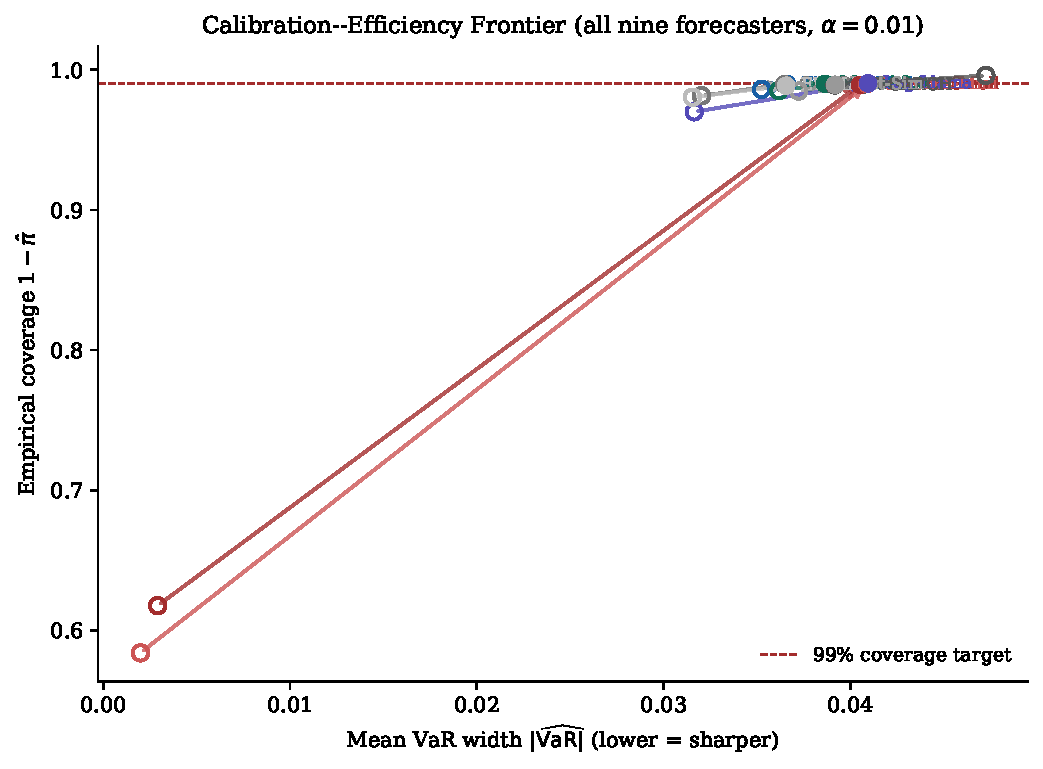
\includegraphics[width=\textwidth]{frontier_all9.pdf}
		\caption{Calibration--efficiency frontier for all nine forecasters at $\alpha = 0.01$. Each arrow traces one forecaster from its raw (hollow) to its conformally corrected (filled) position. Chronos-Small and Chronos-Mini enter from raw coverage ${\approx}60\%$ (replacement regime, shown clipped at 0.55 for display).}
		\label{fig:frontier_all9}
	\end{figure}

\end{document}
